\chapter{CR as Underlay System}
\label{chapter:US}

\section{Introduction}
\subsection{Power control}
Transmission power control

\section{Single cognitive relay}
\begin{figure}[!t]
     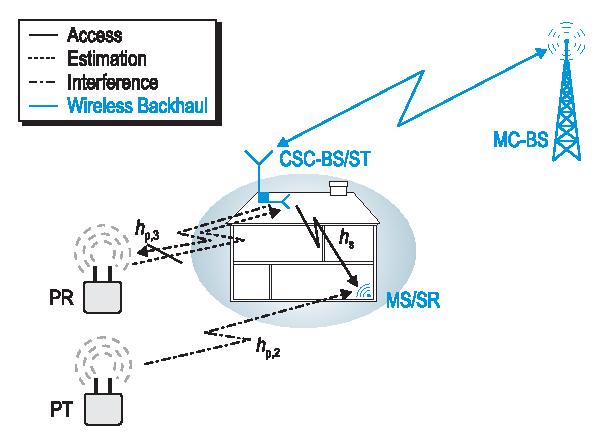
\includegraphics[trim=0cm 0.0cm 0.0cm 0cm,clip=true,width=\columnwidth]{../kapitel04/figures/CR_Scenario_Underlay}
\caption{An illustration of a single \ac{CR} underlay scenario}
\label{fig:Und_Sc}
\end{figure}


%\subsection{Perfect channel estimation}
\subsection{Imperfect channel estimation}




\subsection{Noise uncertainty}
\begin{figure}[!t]
\makeatletter
        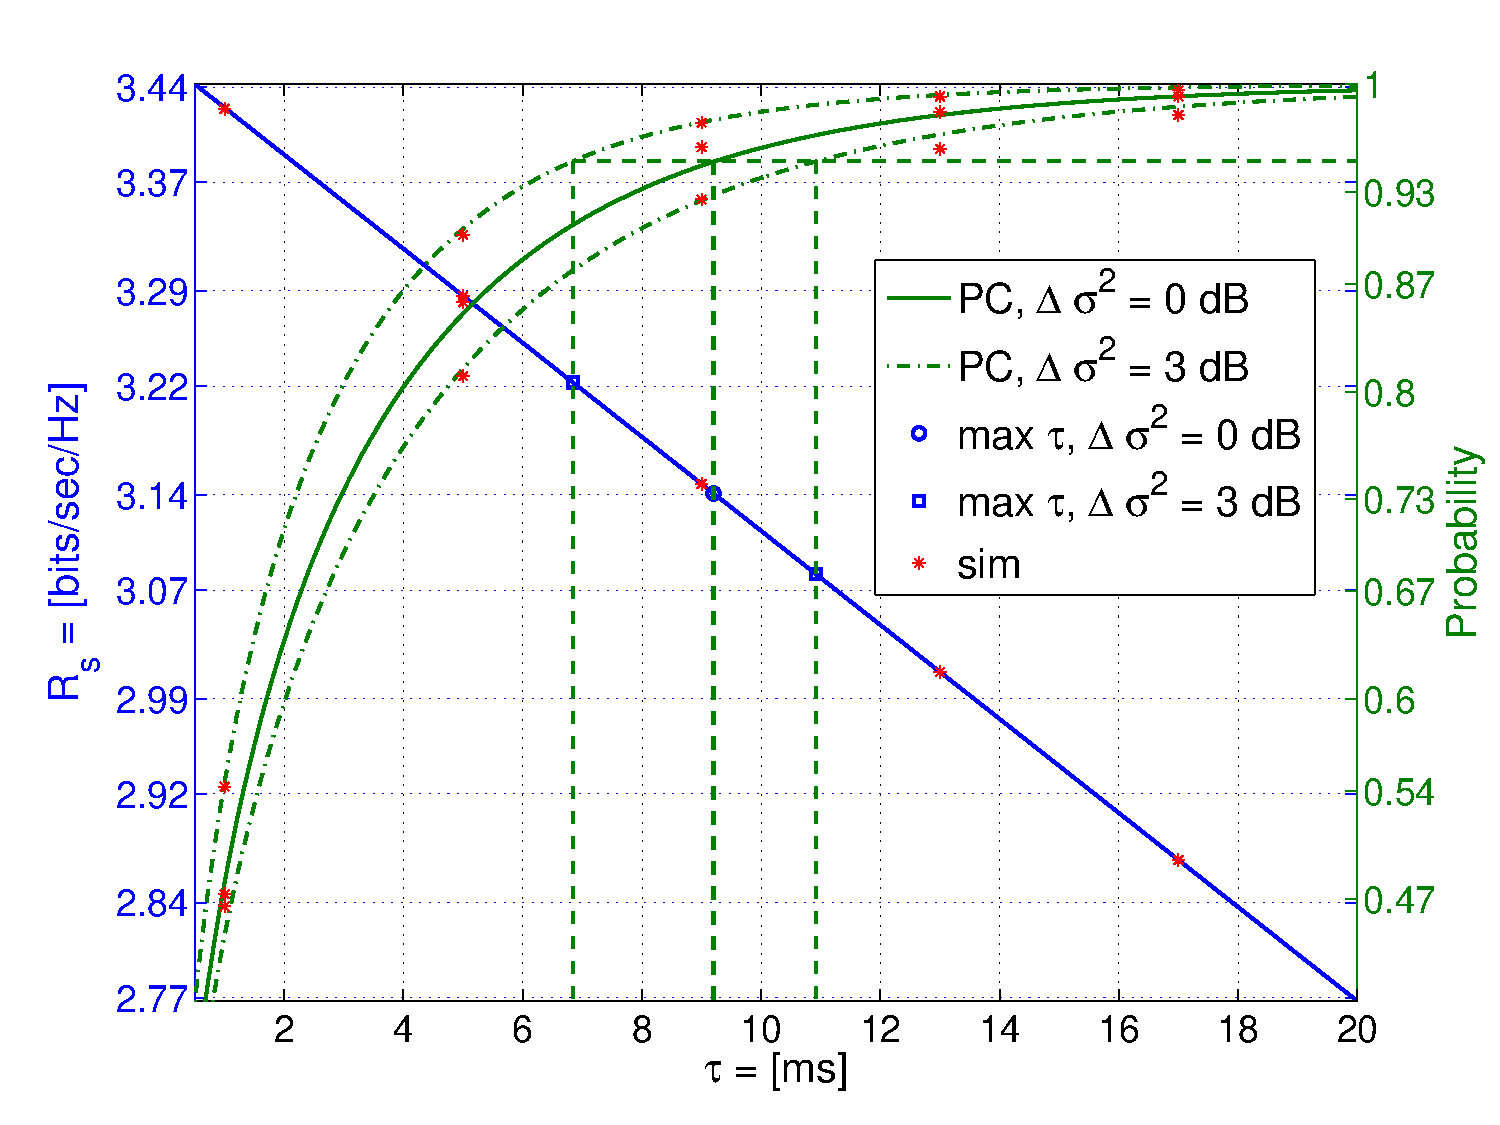
\includegraphics[trim=0.6cm 0.4cm 0.2cm 1.2cm,clip=true,width=\columnwidth]{../kapitel04/figures/fig_thr_est_time_tradeoff_AWGN}
\caption{An illustration of estimation-throughput tradeoff}
\label{fig:ID_OC}
\end{figure}



\section{Cognitive relay networks}
\subsection{System model}

\begin{figure}[!t]
        \centering
        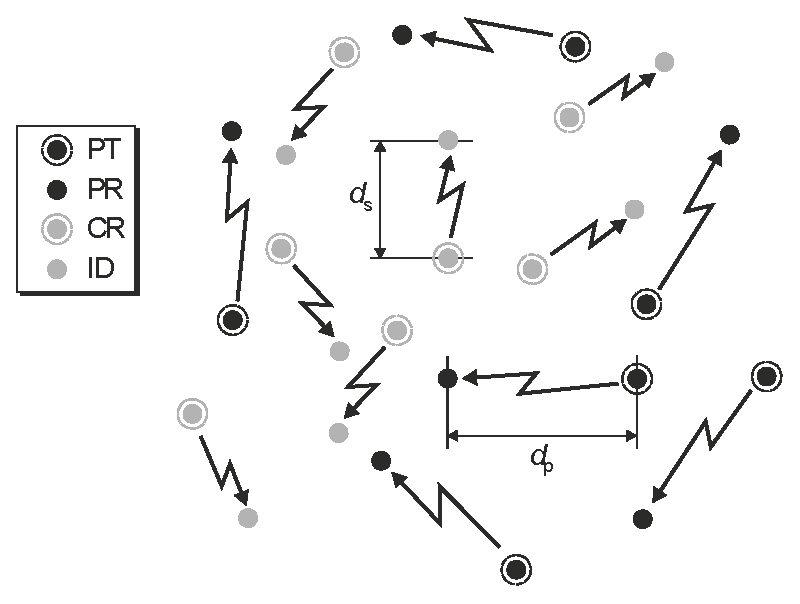
\includegraphics[trim=0.0cm 0.0cm 0.0cm 0.0cm,clip=true,width= 0.85 \columnwidth]{../kapitel04/figures/SGeometry}
        \caption{A realization of a PPP for a cognitive relay network, depicting interference among the primary and secondary nodes.} 
        \label{fig:Int_Sc}
\end{figure}
\cite{Kaushik_PIMRC}

%
%\section{Overview of the TETRA standard}
%\ac{TETRA}\index{TETRA} is an open specification for a digital communication system defined by \ac{ETSI} in 1995. It is intended as a radio link for public safety agencies like police or fire department and will replace legacy analog radio devices. Therefore, the carrier frequency was specified to be in the already existing VHF and UHF bands for \ac{PMR}\index{Public Mobile Radio}. With a bandwidth of \SI{25}{kHz}, two \SI{12.5}{kHz} wide analog FM channels can be replaced by one channel of the new digital system. Due to the TDMA structure with four time slots per channel, the number of users for each channel can be doubled. Furthermore, new features like multicasting and broadcasting, data transmission and encryption, access to the Internet and a better resistance against interferences are added. Although its first draft was released in 1995, the integration of the system in the current radio communication structure for public mobile radio is still ongoing. The European project WINTSEC proposed \ac{SDR} as a way for cost efficient introduction of new communication systems by a software based interoperability with the legacy devices.
%
%This chapter describes the software based development of a TETRA waveform under the aspect of portability. Due to the high complexity of the specification, this work focuses on the user plane of the \ac{V+D} air interface protocol stack. Therefore, \ac{PHY} and \ac{MAC} layers are implemented. For completeness, figure \ref{fig:architecture_VD} shows the architecture of the \ac{V+D} protocol stack for the user plane as well as the higher levels of the control plane. The implemented \ac{PHY} and \ac{MAC} layers are highlighted in gray.
%
%\begin{figure}[htb]
%	\centering
%		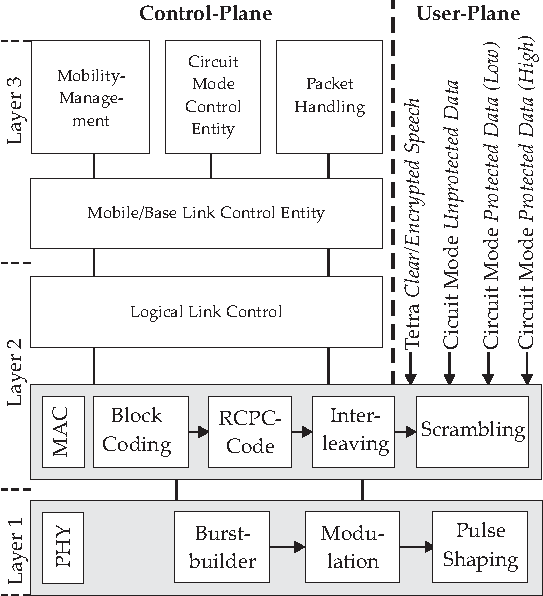
\includegraphics[]{../kapitel04/figures/architecture_VD.pdf}
%	\caption{Architecture of the V+D protocol stack, based on \cite{Steppler}}
%	\label{fig:architecture_VD}
%\end{figure}
%
%The user plane specifies four possible traffic channels for transmitting user data, which are distinguished according to the robustness of channel coding and the data rate as follows\index{Traffic channel}:
%		\begin{description}
% 	 		\item [Traffic CHannel/2.4 (TCH/2.4):]
%				Channel for data transmission with high protection. The bit rate is according to the name \SI{2.4}{kbit/s}
%
% 	 		\item [Traffic CHannel/4.8 (TCH/4.8):]
%				Channel for data transmission with low protection. The bit rate is according to the name \SI{4.8}{kbit/s}
%			
%			\item [Traffic CHannel/7.2 (TCH/7.2):]
% 				Channel for data transmission without protection. The bit rate is according to the name \SI{7.2}{kbit/s}
%
%			\item [Traffic CHannel/Speech (TCH/S):]
%			  Channel for speech transmission, due to the bit rate of the underlying voice codec of \SI{4567}{bit/s}, the TCH/S uses TCH/4.8.
%		\end{description}
%The various traffic channels described above are only logical channels. The mapping from logical to physical channels will be described in the specification of the \ac{PHY} in section \ref{sec:cim_phy}.
%		
%\section{Computational Independent Model}
%\label{sec:TETRA_CIM}
%\index{CIM}
%\subsection{Media Access Control}
%\index{Media Access Control}
%The \ac{MAC} layer of TETRA consists of channel coding\index{Channel coding}, interleaving\index{Interleaving} and scrambling\index{Scrambling} according to figure \ref{fig:architecture_VD}. These operations are shown in more detail in figure \ref{fig:MAC_TETRA} with separation in the different traffic channels. For a complete description of the individual coding and interleaving schemes, five planes are introduced that separate the different processing blocks. In this nomenclature $b_x[k]$ is the bit at position $k$ of plane number $x$. The figure shows furthermore the width of the bit fields, which differs according to the data rate of the different channels. The length of these fields in plane $x$ is named $K_x$. 
%
%\begin{figure}[htb]
%	\centering
%		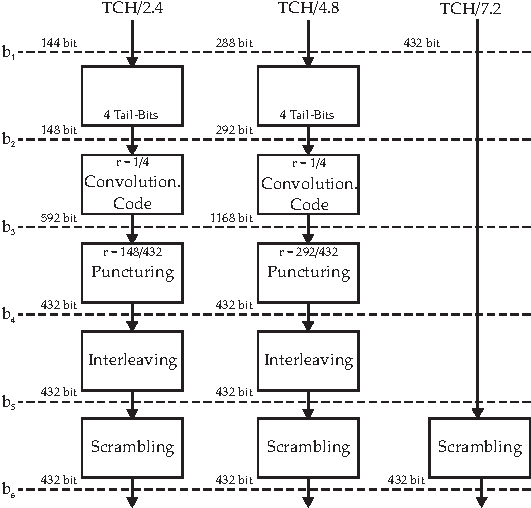
\includegraphics[]{../kapitel04/figures/MAC_TETRA.pdf}
%	\caption{Overview of the encoding and scrambling schemes, used in the transmit side of the traffic channel}
%	\label{fig:MAC_TETRA}
%\end{figure}
%
%To assure that the convolutional encoder ends up in a defined state, the information bits for TCH/2.4 and TCH/4.8 must be extended with four tail bits according to the following clauses:
%
%\begin{equation}
% b_2[k]= 
%\begin{cases}
%	b_1[k] & \text{for} \quad 1 \leq k \leq K_1 \\
%	0			 & \text{for} \quad K_1 < k \leq K_2
%	\end{cases}
%\end{equation}
%
%For the TCH/2.4 the length of the vector is $K_1=144$ while for the TCH/4.8 the length is specified to $K_1=288$. For these channels a zero padding of four bits is inserted due to the register length of four for the following encoding. Therefore, the length of $K_2$ can be determined to be $K_2 = K_1+4$. Due to the fact that the  TCH/7.2 is not protecting its information with channel encoding, neither tail bits nor encoding schemes or interleaving are needed. For the traffic channels TCH/2.4 and TCH/4.8 the convolutional coding is identical. The encoded bits $b_3$ can be calculated by:
%
%\begin{equation}
% b_3[4(k-1)+i]=\sum_{j=0}^{4} b_2[k-j]g_{i,j} \quad \text{for} \quad 
%\begin{cases}
%             &i=1, 2, 3, 4    \\
%             &k=1, 2,..., K_2 \; .
% \end{cases}
%\end{equation}
%
%In this equation, $g_{i,j}$ is the element $j$ at row $i$ of the matrix that can be described by the generator polynomials of the rate $\frac{1}{4}$ mother code:
%
%\begin{table}[!!ht]
%	\centering\begin{tabular}{lcl}
%		$G_1(X)=1+X+X^4$		&$\Rightarrow$	&$g_1=[1 1 0 0 1]$\\
%		$G_2(X)=1+X^2+X^3+X^4$	&$\Rightarrow$	&$g_2=[1 0 1 1 1]$\\
%		$G_3(X)=1+X+X^2+X^4$	&$\Rightarrow$	&$g_3=[1 1 1 0 1]$\\
%		$G_4(X)=1+X+X^3+X^4$	&$\Rightarrow$	&$g_4=[1 1 0 1 1]$\\
%	\end{tabular}\\
%\end{table}
%
%At this point, the traffic channels have different frame lengths. This can also be seen in figure \ref{fig:MAC_TETRA}. The length of the bit field $K_3$ is 592 for the TCH/2.4, 1168 for the TCH/4.8 and 432 for the TCH/7.2. To achieve the specified frame length of $K_4 = 432$ bit, which is equal for all channels, the redundancy of the encoded channels is reduced with different puncturing schemes. The puncturing\index{Puncturing} can be described as follows:
%\begin{equation}
%b_4[k] = b_3[j(k)]
%\label{eq:pun}
%\end{equation}
%
%The index $j$ can be calculated dependent on the index $k$ from the output vector by the following equation for the TCH/2.4: 
%
%\begin{equation}
%	j(k) = 8\left(\left\lfloor \frac{k-1+k_{35}}{6}\right\rfloor \right)+ P_{2.4} \left( k+k_{35} - 6 \cdot \left\lfloor \frac{k-1+k_{35}}{6}\right\rfloor\right),
%\end{equation}
%
%where $\lfloor x \rfloor$ is the floor function\index{Floor function} that rounds down to the largest integer smaller than $x$. The variable $k_x$ is a counter that increments for multiples of $x$. This can be described by
%\begin{equation}
%k_x = \left\lfloor \frac{k-1}{x}\right\rfloor.
%\end{equation}
%
%The mapping of $P_{2.4}$ is depicted in table \ref{tab:Punct_TCH}. For the TCH/4.8 the index $j$ is calculated with
%\begin{equation}
%	j(k) = 8\left(\left\lfloor \frac{k-1+k_{65}}{3}\right\rfloor \right) + P_{4.8} \left( k+k_{65} - 3 \cdot \left\lfloor \frac{k-1+k_{65}}{3}\right\rfloor\right),
%\end{equation}
%
%where the mapping of $P_{4.8}$ is also depicted in table \ref{tab:Punct_TCH}.
%
%\begin{table}[h]
%	\centering
%		\begin{tabular}{c|c|c}
%		\toprule
%			$i$ & $P_{2.4}(i)$ & $P_{4.8}(i)$ \\
%		\midrule
%			1 & 1			& 1 \\
%			2 & 2			& 2 \\
%			3 & 3			& 5 \\
%			4 &	5			&   \\
%			5 &	6			&   \\
%			6 &	7			&   \\
%			\bottomrule
%		\end{tabular}
%		\caption{Mapping of the puncturing scheme for TCH/2.4 and TCH/4.8}
%		\label{tab:Punct_TCH}
%\end{table}
%
%The interleaving mechanism follows the same rule for TCH/2.4 and TCH/4.8 respectively. Therefore the bits are interleaved by
%\begin{equation}
%b_5[k] = b_4\left[ 1+ \left((103 \cdot k) \bmod (432) \right )  \right] \quad \text{for} \quad 1 \leq k \leq 432 \;.
%\label{eq:int_tx}
%\end{equation}
%
%While interleaving is only applied within the convolutional encoded channels, the scrambling mechanism is the same for all traffic channels. It is done by adding a pseudo noise sequence $p[k]$ to the bits:
%\begin{equation}
%b_6[k] = b_5[k] \oplus p[k] \quad \text{for} \quad 1 \leq k \leq 432
%\end{equation}
%
%The scrambling sequence $p[k]$ is generated by a 32 bit wide linear feedback shift register with a connection polynomial of
%
%\begin{eqnarray*}
%c(x) 	&=& \sum_{i=0}^{32}{c_i x^i}\\
%			&=& 1+x+x^2+x^4+x^5+x^7+x^8+x^{10} \\
%			& & +x^{11}+x^{12}+x^{16}+x^{22}+x^{23}+x^{26}+x^{32} \;.
%\end{eqnarray*}
%
%Hereby, the $k$-th bit of the scrambling sequence is given by
%\begin{equation}
%p[k] = \sum_{i=1}^{32}c_i p[k-i].
%\end{equation}
%
%Beside the connection polynomial, the initialization of the register defines the scrambling code. This is done with the \textsc{Extended Colour Code}\index{Extended Colour Code} $e[k]$:
%\begin{equation}
%p[k] = \begin{cases}
%e[1-k]  & \quad \text{for} \quad -29 \leq k \leq 0 \\
%1				& \quad \text{for} \quad -31 \leq k \leq -30 \\
%\end{cases}
%\end{equation}
%The \textsc{Extended Colour Code} consists of 30 bits and describes the mobile station according to figure \ref{fig:ECC}. The first ten bits are defined by the \textsc{Mobile Country Code} which identifies the country where the device is registered. The next 14 bits identify the access net within the country with the \textsc{Mobile Network Code}. The last six bits, finally, represent the \textsc{Colour Code}, which identifies the individual mobile \cite{DigCom_tetra}. To achieve a register length of 32, two defined bits are added.
%
%\begin{figure}[htb]
%	\centering
%		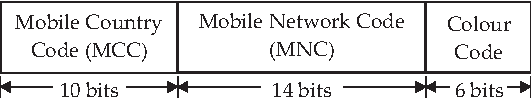
\includegraphics[]{../kapitel04/figures/Extended_Colour_Code.pdf}
%	\caption{Initialization of the scrambling registers with the \textsc{Extended Colour Code}}
%	\label{fig:ECC}
%\end{figure}
%
%
%\subsection{Physical Layer}
%\label{sec:cim_phy}
%\index{Physical layer}
%
%Similar to the well known \ac{GSM} standard, \ac{TETRA} is specified to use a combination of \ac{TDMA} and \ac{FDMA} to give multiple users access to the air interface. A \ac{TDMA} frame in the TETRA system consists of four time slots, for supporting up to four users on a single frequency of \SI{25}{kHz} bandwidth. Uplink and downlink are separated in time and frequency where the various European regulatory organizations agreed on a distance of \SI{10}{MHz} between uplink and downlink carrier. To ease the requirements for a mobile station, uplink and downlink are not only separated in frequency, they are further shifted by two slots in time. Figure \ref{fig:physical_channel} shows the \ac{TDMA}/\ac{FDMA} structure with the combination of \ac{FDD} and \ac{TDD}. The gray boxes show an example of a physical channel, defined with a pair of frequencies (for uplink and downlink carriers) and a corresponding time slot number \cite{ETSI07}. 
%
%\begin{figure}[htb]
%	\centering
%		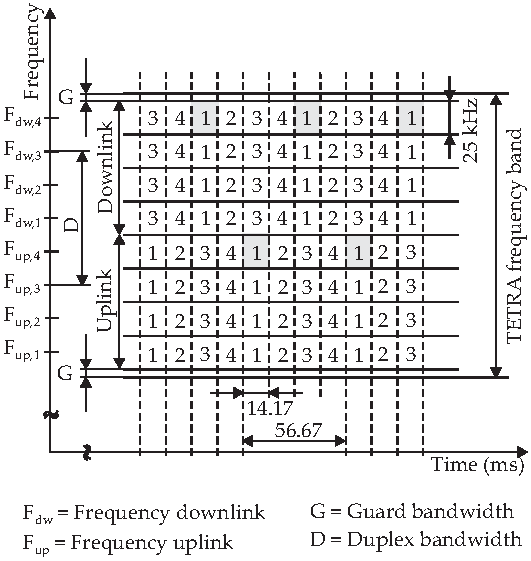
\includegraphics[]{../kapitel04/figures/physical_channel.pdf}
%	\caption{Overview of the FDMA/TDMA structure}
%	\label{fig:physical_channel}
%\end{figure}
%
%In every occupied time slot one burst is transmitted. TETRA specifies four bursts for the downlink and another three bursts for the uplink. With these bursts, control information, synchronization mechanisms and user data can be transmitted. Due to the fact that this work is focused on the user plane, only the bursts containing user data or synchronization information are considered. A \textsc{Normal Uplink Burst} or a \textsc{Normal Downlink Burst} consists of 510 bits and maps the logical traffic channels to the physical channels by extending the coded bits with training sequences, guard intervals and control information. In addition, special synchronization bursts ensure that the mobile station can be synchronized to its frequency and frame structure. Examples of uplink and downlink bursts, specified in the TETRA standard and considered in the \ac{CIM}, are shown in figure \ref{fig:TETRA_bursts}. To achieve a data transmission, the \textsc{Normal Downlink Burst}\index{Normal Downlink Burst} is transmitted. The two blocks with encoded data comprise of the 432 bit long traffic channel, which can be encoded with the error schemes described in the previous section. The broadcast bits, indicated as BBK in figure \ref{fig:TETRA_bursts}, are control information from the \ac{AACH}\index{Access Assignment Channel}. This is a channel that controls the time slot occupation in uplink and downlink. As mentioned previously, this work focuses on the user plane. However, for the sake of completeness the \ac{AACH} is part of the \textsc{Normal Downlink Burst} and has therefore to be implemented. The information for the \ac{AACH} consists of 14 bits that are encoded with a shortened Reed Muller code\index{Reed Muller code}, leading to a coded bit length of 30. The generator matrix can be found in \cite{ETSI07}. The coded bits are scrambled with the scheme described above and form the BBK bits in the \textsc{Normal Downlink Burst}.
%
%
%\begin{figure}[htb]
%	\centering
%		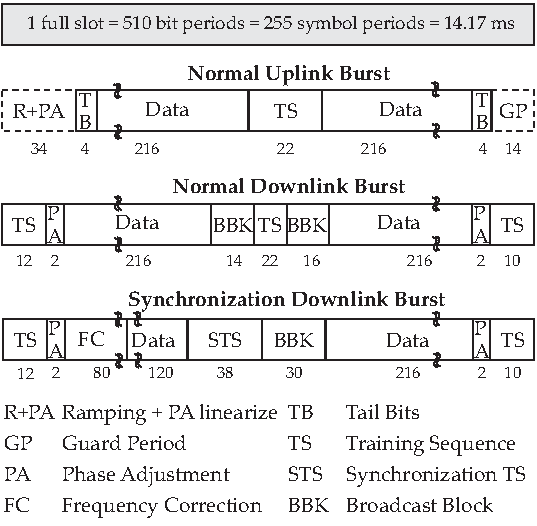
\includegraphics[]{../kapitel04/figures/TETRA_bursts.pdf}
%	\caption{TETRA V+D uplink and downlink burst types}
%	\label{fig:TETRA_bursts}
%\end{figure}
%
%The bits of the bursts are modulated with a \ac{DQPSK}\index{Phase-Shift keying} scheme with a phase offset of $\nicefrac{\pi}{4}$. Due to the fact that a phase rotation must occur between two adjacent symbols, the current symbol $s[k]$ can be calculated dependent on the previous one by
%
%\begin{equation}
%		s[k]=s[k-1]e^{j\phi[k]} \quad \text{with} \quad s[0]=1\;.
%\end{equation}
%
%The phase offset $\phi[k]$ depends on the current symbol and can be determined using table \ref{table:phase_offset}. With these values, no phase shift of $\pm \pi$ occurs, which reduces fluctuations in the magnitude of the complex envelope. This eases the linearization requirements of power amplifiers, especially in mobile devices where power amplifier should be as cheap as possible. The signal trajectory of this modulation scheme is shown on the left hand side in figure \ref{fig:sig_const}. Another advantage of this modulation scheme is that it allows non-coherent demodulation at the receiver, due to the fact that information is not transmitted with the current phase but with the phase offset. Even if the \ac{SNR}\index{Signal-to-Noise Ratio} has to be doubled to achieve the same bit error rate as QPSK, the ease of the synchronization compensates this loss.
%
%\begin{table}[htb]
%\captionabove{Phase offset depending on the actual symbol}\label{table:phase_offset}
%	\centering\begin{tabular}{cc|c|c}
%	\toprule
%	Bit 2	& Bit 1	& Symbol	& $\phi$[k] \\
%	\midrule
%	$1$	& $1$	& $3$	& - $\frac{3\pi}{4}$  \\
%	$0$	& $1$	& $1$	& + $\frac{3\pi}{4}$  \\
%	$0$	& $0$	& $0$	& - $\frac{\pi}{4}$  \\
%	$1$	& $0$	& $2$	& + $\frac{\pi}{4}$  \\
%	\bottomrule
%	\end{tabular}
%\end{table}
%
%To generate the transmit signal $s_\text{tx}(t)$, the discrete time symbols $s[k]$ are filtered with a time continuous pulse shaping\index{Pulse shaping} filter $g_{\text{RRC}}(t)$. This can be described as follows: 
%
%\begin{equation}
%		s_\text{tx}(t)=\sum_{k=0}^{K}{s[k] \cdot g_{\text{RRC}}(t-kT_\text{sym})},
%\end{equation}
%
%where $T_\text{sym}$ is the symbol duration of \SI{55.56}{\micro s} and $K$ is the maximum number of symbols. The impulse response of the pulse shaping filter $g_{\text{RRC}}(t)$ is obtained by the inverse Fourier transform of a square root raised cosine\index{Root raised cosine} spectrum $G_{\text{RRC}}(f)$ with roll-off factor $\alpha$  defined as
%\begin{align}	
%G_{\text{RRC}}(f)=
%\begin{cases} 
%1,     & |f| \leq \frac{1-\alpha}{2T_{\text{sym}}} \\
%\cos \left(\frac{\pi T_{\text{sym}}}{2 \alpha}\left( |f| - \frac{1 - \alpha}{2 T_{\text{sym}}}\right)\right), 
%      & \frac{1-\alpha}{2T_{\text{sym}}} < |f| \leq \frac{1+\alpha}{2T_{\text{sym}}} \\
%0,     & |f| > \frac{1+\alpha}{2T_{\text{sym}}}\;.
%\end{cases}
%\label{eq:g_rrc_f}
%\end{align}
%
%TETRA specifies $\alpha = 0.35$ and offers the possibility to implement a time limited version of $g_\text{RRC}(t)$ that fulfills the constraints of modulation accuracy and adjacent channel attenuation. Therefore, the sequence of  complex symbols $s[k]$ must be interpolated by a factor of $I_\text{RRC}$ and furthermore filtered with a discrete time realization of the root raised cosine filter. This is identical to the sampling of the time continuous transmit function $s_\text{tx}(t)$ with sampling rate $I_\text{RRC}/T_\text{sym}$. Hence, the discrete time signal of the transmit sequence can be described as
%
%\begin{equation}
%s_\text{tx}\left(i \cdot \frac{T_\text{sym}}{I_\text{RRC}}\right)  = \sum_{k=0}^{K}{s[k]g_{\text{RRC}}\left(i \cdot \frac{T_\text{sym}}{I_\text{RRC}}-kT_\text{sym}\right)}\;.
%\end{equation}
%
%The design of the filter $g_\text{RRC}(\cdot)$ is platform specific due to the sample rate conversion. Therefore it is part of the \ac{PSM}. However, it has to be mentioned that the pulse shaping filter results in larger fluctuations of the complex envelope and hence a smaller hole of the signal trajectory in the complex plane. This effect is shown on the right hand side of figure \ref{fig:sig_const}.
%
%\begin{figure}[htb]
%	\centering
%		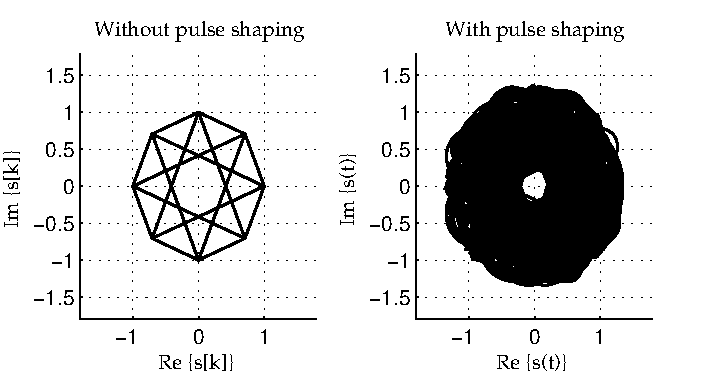
\includegraphics[width=1.00\textwidth]{../kapitel04/figures/sig_const.pdf}
%	\caption{Signal trajectory of the $\frac{\pi}{4}$-DQPSK modulation scheme}
%	\label{fig:sig_const}
%\end{figure}
%
%Table \ref{table:TETRA_overview} summarizes the key parameters of the TETRA system.
%
%\begin{table}[htb]
%\captionabove{Overview of the TETRA system parameter}\label{table:TETRA_overview}
%	\centering\begin{tabular}{cccc}
%	\toprule
%	Parameter					& Value \\
%	\midrule
%	Carrier frequency	& 400 MHz	 \\
%	Bandwidth					& 25 kHz \\
%	Media access			& TDMA/FDMA \\
%	Duplex mode				& TDD/FDD \\
%	Users per carrier	& 4 \\
%	Modulation				& $\frac{\pi}{4}$-DQPSK \\
%	Channel coding		& RCPC \\
%	Symbol rate				& 18 kBaud/s \\
%	Bits per slot			& 510 \\
%	Frame duration		& 56.67 ms \\
%	Bursts per frame	& 4 \\
%	Burst duration		& 14.167 ms \\
%	Pulse shaping			& RRC with 0.35 rolloff \\
%	Data rate					& up to 28.8 kbit/s \\
%	\bottomrule
%	\end{tabular}
%\end{table}
%
%\section{Platform Independent Model}
%\index{CIM}
%\label{sec:PIM_TETRA}
%The Platform Independent Model of TETRA is the implementation of the transmit path as described in the \ac{CIM} in the previous section \ref{sec:TETRA_CIM}. Furthermore, the receive side is implemented with the synchronization of time, frequency and frame, which is not described in the \ac{CIM}.
%
%\subsection{Transmitter}
%The input of the transmitter is a vector with random bits generated by a \ac{PN} sequence and is used as information data. The length of this array depends on the traffic channel and can vary from 144 bits for the TCH/2.4, over 288 bits for the TCH/4.8 to 432 bits for the TCH/7.2. The encoding depends also on the traffic channel and assures an output length of 432 bits, independent of the channel's data rate. The scrambling with the \textsc{Extended Colour Code} is similar for all channels. It is assumed that the initialization of the register is already known at transmit and receive side.
%
%Another input for the transmitter is the 14 bit wide vector for the control channel (AACH). It has to be mentioned that this channel also transmits random bits. Therefore, no control or configuration is applied from the information of the broadcast channel. The control channel is encoded with a shortened Reed Muller code and scrambled with the same pseudo noise sequence as the traffic channel. The burst builder shown in figure \ref{fig:PIM_Tx} integrates the encoded data fields in a \textsc{Normal Downlink Burst} as defined by the TETRA specification and adds a \textsc{Synchronization Downlink Burst} after 18 regular bursts. This synchronization burst is needed for the frequency synchronization in the receiver. The frame size for the implementation is according to the TETRA burst length set to 510. These bits are modulated with the described $\frac{\pi}{4}$-\ac{DQPSK} modulation scheme to 255 complex symbols. The pulse shaping filter that must fulfill the root raised cosine spectrum finalizes the transmit side. 
%
%\begin{figure}[htb]
%	\centering
%		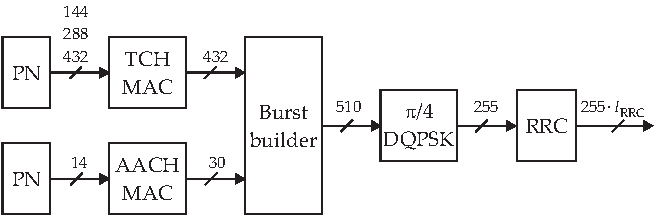
\includegraphics[width=1.00\textwidth]{../kapitel04/figures/PIM_Tx.pdf}
%	\caption{PIM of the TETRA transmit path}
%	\label{fig:PIM_Tx}
%\end{figure}
%
%
%The realization of the \ac{RRC}\index{Root raised cosine} transmit filter as an \ac{FIR} filter can be determined by two parameters: the interpolation factor $I_\text{RRC}$ and the group delay $D_\text{RRC}$. The third parameter, the roll-off factor is already specified in the standard to $\alpha = 0.35$.  According to the symbol rate of \SI{18}{kBaud/s} the symbol time can be determined to $T_\text{sym}$ = \SI{55.56}{\micro s}. The impulse response of an \ac{RRC} filter is according to \cite{Kammeyer}
%
%\begin{equation}
%g_\text{RRC}(t) = 4 \alpha \frac{\cos \left((1+\alpha)\pi \frac{t}{T_\text{sym}} \right) + \frac{\sin \left( (1-\alpha)\pi \frac{t}{T_\text{sym}}\right)}{4 \alpha \frac{t}{T_\text{sym}}}}{\pi \sqrt{T_\text{sym}} \left(1-\left(4 \alpha \frac{t}{T_\text{sym}} \right)^2 \right)}\;.
%\label{eq:g_rrc_t}
%\end{equation}
%
%The discrete time realization of this filter response can be described with the interpolation factor $I_\text{RRC}$ as follows:
%\begin{equation}
%g_\text{RRC}\left( i \cdot \frac{T_\text{sym}}{I_\text{RRC}} \right) = 4 \alpha \frac{\cos \left((1+\alpha)\pi \frac{i}{I_\text{RRC}} \right) + \frac{\sin \left( (1-\alpha)\pi \frac{i}{I_\text{RRC}}\right)}{4 \alpha \frac{i}{I_\text{RRC}}}}{\pi \sqrt{T_\text{sym}} \left(1-\left(4 \alpha \frac{i}{I_\text{RRC}} \right)^2 \right)}
%\end{equation}
%
%Due to the fact that this filter is defined for infinite values of $i$, a time limited version of $g_\text{RRC}(\cdot)$ must be applied and the impulse response must be delayed to achieve a causal filter. The group delay $D_\text{RRC}$ describes the number of symbol durations the impulse response must be shifted and is therefore the implicit parameter of the rectangular window function $w[i]$ with
%
%\begin{equation}
%w[i] = \begin{cases}
%1 & \left |i  \right | \leq D_\text{RRC} \cdot I_\text{RRC} \\
%0 & \left |i  \right | > D_\text{RRC} \cdot I_\text{RRC}.
%\end{cases}
%\end{equation}
%
%The time limited realization of the filter can be described as follows:
%\begin{equation}
%g_\text{RRC,w}\left( i \cdot \frac{T_\text{sym}}{I_\text{RRC}} \right) = g_\text{RRC}\left( i \cdot \frac{T_\text{sym}}{I_\text{RRC}} \right) \cdot w[i]
%\end{equation}
%
%With the multiplication of the window function, the filter length can be determined to $2D_\text{RRC}I_\text{RRC}+1$ and is therefore proportional to the group delay. The performance loss of this filter due to the windowing can be evaluated by the relative energy loss that can be calculated as follows: 
%
%\begin{equation}
%E_\text{rel} = \frac{E_\text{RRC}-E_\text{RRC,w}}{E_\text{RRC}},
%\end{equation}
%
%where the energy of an RRC impulse response can be easily calculated with the impulse response of a raised cosine filter $g_\text{RC}[i]$:
%\begin{eqnarray}
%E_\text{RRC} & = & g_\text{RRC}^*[-i] * g_\text{RRC}[i] \quad |_{i=0} \\
%						& = & \frac{I_\text{RRC}}{T_\text{sym}} \cdot g_\text{RC}[i] \quad |_{i=0} \\
%						& = & \frac{I_\text{RRC}}{T_\text{sym}}
%\end{eqnarray}
%
%The relation of the energies can be determined to:
%\begin{equation}
%E_\text{rel} = 1- \sum_{i=-D_\text{RRC} \cdot I_\text{RRC}}^{D_\text{RRC} \cdot I_\text{RRC}} \left| 4 \alpha \frac{\cos \left((1+\alpha)\pi \frac{i}{I_\text{RRC}} \right) + \frac{\sin \left( (1-\alpha)\pi \frac{i}{I_\text{RRC}}\right)}{4 \alpha \frac{i}{I_\text{RRC}}}}{\pi \sqrt{T_\text{sym}} \left(1-\left(4 \alpha \frac{i}{I_\text{RRC}} \right)^2 \right)}\right|^2
%\end{equation}
%
%Figure \ref{fig:RRC_group_delay} shows the relative energy loss $E_\text{rel}$ in relation to the group delay $D_\text{RRC}$. To achieve an energy loss less than \SI{0.01}{\%} a group delay of six was chosen in combination with an interpolation factor of $I_\text{RRC} = 64$. The chosen parameters result in 769 taps for one filter and the signal processing period for one frame is about \SI{1.5}{ms} on an Intel P8400 processor with a clock frequency of \SI{2.28}{GHz}. Even if this filter length is not feasible for a real time implementation, the combination between filter accuracy and simulation time is acceptable.
%\begin{figure}[htb]
%	\centering
%		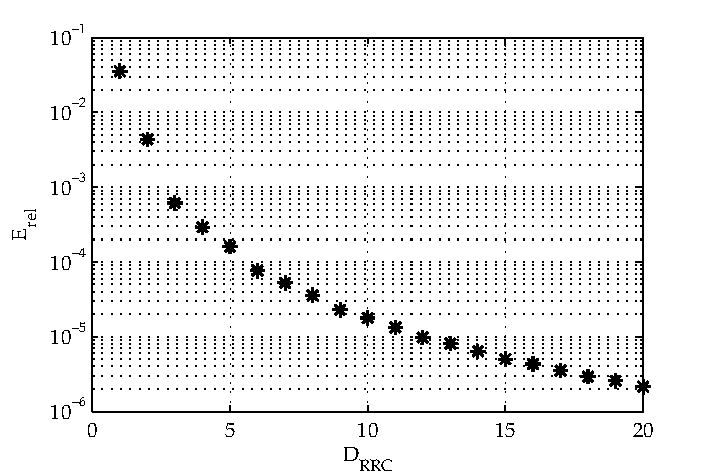
\includegraphics[width=1.00\textwidth]{../kapitel04/figures/RRC_group_delay.pdf}
%	\caption{Relative energy loss of a windowed realization of an RRC in dependence of the group delay $D_\text{RRC}$}
%	\label{fig:RRC_group_delay}
%\end{figure}
%
%
%
%\subsection{Channel}
%\index{Channel}
%For the evaluation of the synchronization algorithms, a channel must be simulated. This channel behaves like a virtual front end and adds a white Gaussian noise signal $n(t)$. The input of the channel consists of a vector comprising the interpolated and filtered symbols $s_\text{tx}(t)$ with the TETRA burst length multiplied with the interpolation factor $I_\text{RRC}$. To introduce channel delay, a fixed latency of $N$ symbols is applied. Hence, a vector comprises two partial TETRA bursts and the receiver has to detect the beginning of a burst. To simulate the different clock frequencies of transmitter and receiver, another delay $\epsilon$ is inserted. In contrast to the first delay, the time shift is not fixed and varies over time. With these operations, the channel can be described as follows:
%\begin{equation}
%r_\text{rx}(t) = s_\text{tx}\left( t-N T_\text{sym} - \epsilon(t) \right) + n(t)
%\end{equation}
%
%Due to the discrete time realization of the \ac{PIM}, the received signal is given by
%\begin{equation}
%r_\text{rx}\left( i \cdot \frac{T_\text{sym}}{I_\text{RRC}} \right) = s_\text{tx}\left(i \cdot \frac{T_\text{sym}}{I_\text{RRC}} -N T_\text{sym} - \epsilon\left( i \cdot \frac{T_\text{sym}}{I_\text{RRC}} \right) \right) + n\left( i \cdot \frac{T_\text{sym}}{I_\text{RRC}} \right).
%\end{equation}
%
%Another effect of the asynchronous local oscillators on the transmitter and receiver is the offset of the carrier frequency $\nu$ and the phase offset $\varphi$. These RF impairments are simulated by the multiplication with a complex harmonic wave. Under the assumption that no time and symbol offset occurs, the receive signal $r_\text{rx}(\cdot)$ can be determined by
% 
%\begin{equation}
%r_\text{rx} \left( i \cdot \frac{T_\text{sym}}{I_\text{RRC}} \right) = s_\text{tx}\left(i \cdot \frac{T_\text{sym}}{I_\text{RRC}} \right)  \cdot e^{j2 \pi \left(\nu \cdot i \cdot \frac{T_\text{sym}}{I_\text{RRC}} +\varphi \right)} + n\left( i \cdot \frac{T_\text{sym}}{I_\text{RRC}} \right).
%\end{equation}
%
%A more detailed description of this channel as a virtual front end can be found in \cite{wnitl}.
% 
%\begin{figure}[htb]
%	\centering
%		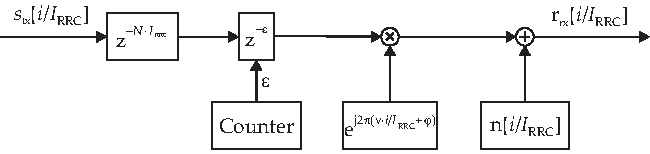
\includegraphics{../kapitel04/figures/channel.pdf}
%	\caption{Structure of the channel, which works as a virtual front end}
%	\label{fig:channel}
%\end{figure}
%
%\subsection{Time Synchronization in TETRA}
%\index{Time synchronization}
%
%To minimize the influence of the additive white Gaussian noise $n(\cdot)$, the received signal $r_\text{rx}(\cdot)$ is filtered with the root raised cosine filter, which is also the matched filter to
%
%\begin{equation}
%r\left( i \cdot \frac{T_\text{sym}}{I_\text{RRC}}\right) = r_\text{rx} \left( i \cdot \frac{T_\text{sym}}{I_\text{RRC}} \right) * g_{\text{RRC}} \left( i \cdot \frac{T_\text{sym}}{I_\text{RRC}} \right).
%\end{equation}
%
%Prior to downsampling, the timing error $\epsilon$ must be determined and corrected. This is done by a square timing error detector as proposed by Oerder in \cite{oerder}. By calculating the square of the absolute value of the received and filtered signal $r(\cdot)$, there are linear distortions leading to spectral peaks at multiples of the system's symbol rate, which include the delay information. The squared receive signal $x[i]$ can be expressed by
%
%\begin{equation}
%x[i] = \left|r\left( i \cdot \frac{T_\text{sym}}{I_\text{RRC}}\right) \right|^2.
%\end{equation}
%
%Figure \ref{fig:square_time} shows the spectrum of the signal $x[i]$. The mentioned spectral lines at multiples of \SI{18}{kHz} indicate the symbol rate. The time delay in the symbol rate is now transformed into a phase shift. Therefore, the delay can be determined by calculating the phase rotation in the spectral domain at the frequency of the symbol rate. By assuming that the timing error is constant over $L$ symbols, the Fourier transform can be applied over $L \cdot I_\text{RRC}$ samples. Due to the fact that only the Fourier coefficient at the symbol rate is needed for the timing error, it can be calculated as follows:
%
%\begin{equation}
%X[m] =  \sum_{i=mLI_\text{RRC}}^{(m+1)LI_\text{RRC}-1} x[i] e^{-j 2 \pi i/I_\text{RRC}}
%\end{equation}
%
%
%\begin{figure}[htb]
%	\centering
%		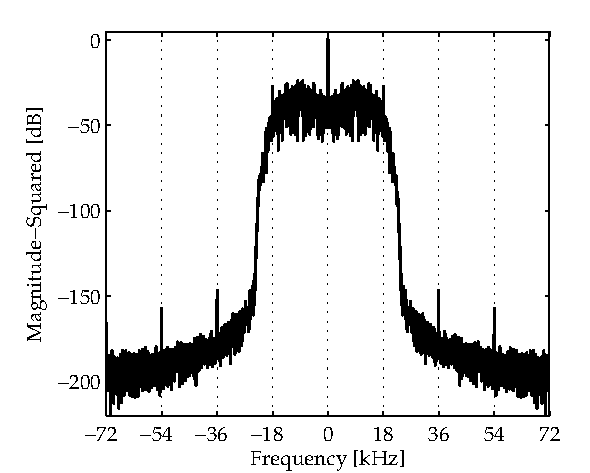
\includegraphics{../kapitel04/figures/square_time.pdf}
%	\caption{Spectrum of the squared magnitude of the receive signal}
%	\label{fig:square_time}
%\end{figure}
%
%Therefore, the timing error $\epsilon$ can be determined by
%
%\begin{equation}
%\epsilon[m] = - \frac{1}{2\pi} \arg \left\{X[m]\right\}\;.
%\end{equation}
%
%It has to be mentioned that the choices of several parameters such as the interpolation factor $I_\text{RRC}$ or the assumption that the timing error is constant over $L$ symbols, depends on the underlying platform. Therefore, these parameters will be discussed in the \ac{PSM}.  
%
%
%\subsection{Frequency Synchronization}
%\index{Frequency synchronization}
%
%The frequency offset is determined by using the 19 symbol wide \textsc{Synchronization Training Sequence}\index{Synchronization Training Sequence} and the 40 symbol wide \textsc{Frequency Correction Field}\index{Frequency Correction Field} as shown in figure \ref{fig:TETRA_bursts}. According to the specification, the \textsc{Synchronization Downlink Burst}\index{Synchronization Downlink Burst} is sent after 18 \textsc{Normal Downlink Bursts}. To detect the \textsc{Synchronization Downlink Burst} the incoming symbols are correlated with the following two training sequences: the \textsc{Frequency Correction Field} and the \textsc{Synchronization Training Sequence}. However, by assuming a frequency offset, the peak of the correlation would disappear in the noise. A possibility to circumvent this is to build the product of the incoming symbol with the conjugate complex of the previous symbol. This transforms the frequency offset to a phase offset. The signal is then correlated with the training sequences and the peak remains detectable for frequency offsets as shown in figure \ref{fig:freq_peak}.
%
%The position of the peak leads to the position of the \textsc{Frequency Correction Field}, which consists of the following bits: 
%
%\begin{equation*}
%FC = [\underbrace{1,1,...,1,1}_{8},\underbrace{0,0,...,0,0}_{64},\underbrace{1,1,...,1,1}_{8}]
%\end{equation*}
%
%The zero bits in the middle of the field lead to a phase offset of $\nicefrac{\pi}{4}$ between two symbols. With this information, the frequency offset can be evaluated by
%
%\begin{equation}
%r(k \cdot T_\text{sym}) \stackrel{!}{=} r((k-1)\cdot T_\text{sym}) e^{j\pi/4} \quad \text{for} \quad k=FC_5 \dots FC_{36}\;.
%\end{equation}
%
%In this equation, $FC_x$ represents the position of symbol number $x$ in the \textsc{Frequency Correction Field} inside the symbol stream. With the following equation:
%
%\begin{equation}
%\hat{\nu} = \frac{1}{2\pi} \cdot \left( \frac{1}{32}\sum_{k=\text{FC}_5}^{\text{FC}_{36}}\arg \left\{r(k \cdot T_\text{sym})\right\} - \arg \left\{r((k-1)\cdot T_\text{sym})\right\} -  \frac{\pi}{4} \right),
%\end{equation}
%
%a frequency offset in the range of \SI{-9}{kHz} to \SI{9}{kHz} can be evaluated. Higher frequency offsets lead to errors due to phase ambiguities. Therefore, frequency offset acquisition algorithms have to be implemented. However, this depends on the platform specific offset and is therefore not taken into account in the \ac{PIM}. Figure \ref{fig:freq_peak} shows the correlation with the known sequences for finding the \textsc{Frequency Correction Field}. The input signal has a signal to noise ratio of SNR = \SI{20}{dB} and a frequency offset of $\nu$ = \SI{1}{kHz}.
%
%
%\begin{figure}[htb]
%	\centering
%		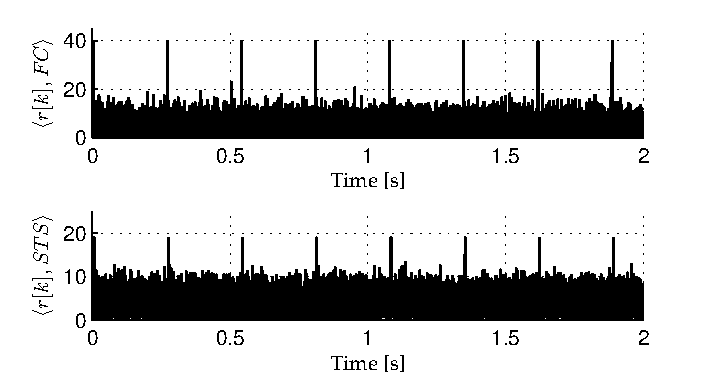
\includegraphics[width=1.00\textwidth]{../kapitel04/figures/freq_peak.pdf}
%	\caption{Correlation of the receive signal $r[k]$ with the synchronization sequences: \textsc{Synchronization Training Sequence} (STS) and \textsc{Frequency Correction Field} (FC)}
%	\label{fig:freq_peak}
%\end{figure}
%
%The frequency offset signal is an error compensation signal in the demodulation. Due to the incoherent demodulation of the signal, the angle of the actual signal is subtracted from the angle of the last symbol. This means that the frequency offset can be regarded as an angle offset between two symbols, leading to another subtraction of the phase offset. With this method, a complex multiplication can be replaced by a simple real addition.
%
%A phase synchronization is not necessary. The differential modulation scheme includes the information on the phase difference between two adjacent symbols. Therefore, no knowledge of the absolute phase position is needed.
%
%\subsection{Frame Synchronization}
%\index{Frame synchronization}
%The output of the demodulator is a bit stream without information about the embedded bursts. Therefore, the frame synchronization extracts the traffic and control channels from the bit stream. To find the logical channels inside the stream, every burst includes training sequences as shown in figure \ref{fig:TETRA_bursts}. When receiving data from the \textsc{Normal Continuous Downlink Burst}, the frame synchronization searches the bit stream for the \textsc{Training Sequence 1} (TS1) and \textsc{Training Sequence 3} (TS3). These fields indicate the start and stop of the traffic and the control channel. The output is a 432 bit long vector, comprising the \ac{TCH} and a 30 bit long vector with the \ac{AACH}. The receiver for the physical layer is shown in figure \ref{fig:tetra_rx_pim} with a matched filter, time synchronization, frequency synchronization and frame synchronization.
%
%\begin{figure}[htb]
%	\centering
%		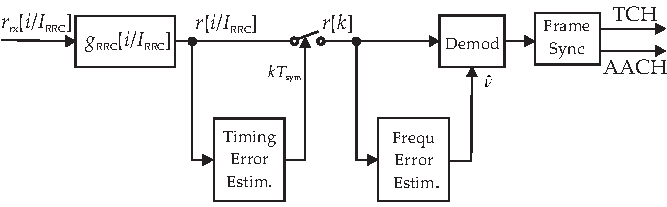
\includegraphics{../kapitel04/figures/tetra_rx_pim.pdf}
%	\caption{Overview of the \ac{PIM} of the receiving \ac{PHY}}
%	\label{fig:tetra_rx_pim}
%\end{figure}
%
%\subsection{MAC receiver}
%The input of the MAC receiver comprises two vectors: the 432 bit long \ac{TCH} and the 30 bit long \ac{AACH}. Since both channels are encoded differently, two receivers have to be used that work in parallel. The first operation in the \ac{TCH} receiver is descrambling. Due to the fact that an additive scrambler was used in the transmit path, the descrambling can be achieved by a second addition with the pseudo noise sequence $p[k]$. To generate the same sequence as in the transmitter, the initialization of the register with the \textsc{Extended Colour Code}\index{Extended Colour Code} must be known at the receiver. The descrambling can be described by
%\begin{equation}
%\hat{b}_5[k] = \hat{b}_6[k] + p[k] \quad \text{for} \quad 1 \leq k \leq 432\;,
%\end{equation}
%
%where $\hat{b}_x[k]$ represents the approximated bit at position $k$ of the plane $x$ as indicated in the transmit side by figure \ref{fig:MAC_TETRA}.
%
%In case of the TCH/7.2, the descrambled bits are the information bits with
%\begin{equation}
%\hat{b}_1[k] = \hat{b}_5[k]\;.
%\end{equation}
%
%No decoding is applied, however, the bits of the other traffic channels must be descrambled. According to the interleaving scheme, which was described in equation (\ref{eq:int_tx}), the inverse element of 103 has to be determined. It can be shown that 151 is the inverse element to 103 when holding the condition
%\begin{equation}
%(151 \cdot 103) \mod 432  = 1\;.
%\end{equation}
%
%The de-interleaving can be applied as follows:
%\begin{equation}
%\hat{b}_4[k] = \hat{b}_5\left[ 1+ \left( 151 \left(k-1\right)-1\right) \bmod (432)  \right] \quad \text{for} \quad 1 \leq k \leq 432
%\label{eq:deint}
%\end{equation} 
%
%The time shifts are necessary because the range of values have to be mapped from the modulo 432 interval $[0,431]$ to the interval $[1,432]$. The now de-interleaved data are decoded, according to the dedicated traffic channel. The lengths of 592 for the TCH/2.4 and 1168 for the TCH/4.8 can be achieved by inserting random bits at the positions where information data were dropped, according to the scheme described in equation (\ref{eq:pun}) and table \ref{tab:Punct_TCH}. Due to the fact that there is no information about the inserted data, values of 0.5 are inserted.
%
%The decoding is achieved with a Viterbi algorithm\index{Viterbi decoding}. Since the \ac{PIM} is not a real-time implementation, the traceback length of the Viterbi decoder can be set to the frame length, leading to the best error correction performance. However, due to the applied scrambling of the data, the Viterbi decoder works in a hard decision mode. The only bits with reliability values are the punctured bits, which are included with values of 0.5. An advantage of the hard decision decoding is the reduced memory usage. This yields in a loss of approximately \SI{2.5}{dB} in the SNR compared to soft decision decoding \cite{Bossert}.
%
%The 30 bit wide data field of the \ac{AACH} is descrambled with the same sequence used for the traffic channels. The decoding is achieved with the parity check matrix, which is used to calculate the syndrome vector. Since the syndrome depends only on the error vector and not on the code word, it can be mapped to an error pattern. However, due to the fact that there are $2^{16}$ different syndromes, only pattern errors with one bit error are searched. This eases the implementation and is a valid expectation. The probability that more than one bit is wrong in the 30 bit long \ac{AACH} receive vector can be calculated with the bit error rate of the uncoded data $P_b$ to
%
%\begin{equation}
%P_\text{AACH} = 1-\left(\left(1-P_b\right)^{30}+30\left(1-P_b\right)^{29} \cdot P_b\right)\;.
%\end{equation}
%
%Assuming a bit error rate of $P_b = 0.01$ on the channel, the probability that the AACH would be decoded incorrectly is \SI{3.6}{\%}.
%
%
%\section{Platform Specific Model for the USRP}
%\label{sec:PSM_USRP}
%\index{Platform Specific Model}
%\index{USRP}
%
%\subsection{Separation on different processing elements}
%As described in section \ref{sec:USRP}, the platform consists of an FPGA on the USRP and a GPP. Due to the fact that the FPGA is relatively small and without hardware multipliers, most of the signal processing should be located on the GPP. The sample rate conversion from symbol rate to \ac{DAC} rate and vice versa should be done in the FPGA. Another limitation of the FPGA is the fixed clock frequency of \SI{64}{MHz}, leading to sampling rates that are only integer divisions of this rate. In the following the resampling for the transmit side is described. As introduced in section \ref{sec:PIM_TETRA}, the symbol time interval is denoted by $T_\text{sym}$. The sampling rate of the \ac{DAC} is given by $f_s = 1/T_s$. The TETRA symbol rate is according to table \ref{table:TETRA_overview} $f_\text{sym} = \SI{18}{kHz}$. The input rate of the \acp{DAC} is $f_s = \SI{32}{MHz}$. With these data, a resampling factor $R$ can be determined with the following factors of interpolation and decimation:
%
%\begin{equation}
%	R = \frac{f_s}{f_\text{sym}}=\frac{\SI{32}{MHz}}{\SI{18}{kHz}} = \frac{2^7\cdot 5^3}{3^2}
%\label{eq:res_usrp}
%\end{equation}
%
%Due to the architecture of the platform, the FPGA is only able to work with an upsampling factor of integer numbers. This leads to a resampling over two stages: the first resampling stage is realized in the GPP, while the second stage is done in the FPGA with an interpolation to achieve the DAC rate of \SI{32}{MHz}. This yields the factors
%
%\begin{equation}
%	R = \frac{I_\text{GPP}}{D_\text{GPP}}\cdot I_\text{FPGA} = \frac{I_\text{FIR}}{D_\text{FIR}}\cdot I_\text{CIC}\;.
%\label{eq:r}
%\end{equation}
%
%The FPGA provides no multipliers and should perform a high sampling rate conversion. Therefore, a \ac{CIC} interpolation filter as described in \cite{hogenauer} is needed. CIC filters\index{CIC filter} are a class of digital filters that achieve decimation\index{Decimation} and interpolation\index{Interpolation} without any multipliers. The hardware efficient implementation is furthermore favored by the highly symmetrical structure, comprising cascaded integrator and comb filter pairs \cite{cic_comp}. However, CIC filters have two major disadvantages. The first is that the internal word width increases with the number of stages. However, due to the fact that the FPGA is able to work on data words with arbitrary lengths, this is not a problem in this realization. The second disadvantage is the passband of the filter, which is not flat. To circumvent this problem, an \ac{FIR} filter has to be designed on the GPP that compensates the CIC frequency response in the desired band. The design of these filters is described in the next section.
%
%Figure \ref{fig:tetra_rx_sampling_USRP} shows the separation of the resampling on the USRP. The remaining part of the transmitter on the GPP is not shown. The resampling on the receive side has two differences in comparison to the concept of the transmit side. The decimation factors on the receiver are represented with the letter $I$, while the interpolation factors are described with the letter $D$. This is due to the fact that the same interpolation and decimation rates are used on the transmit and receive side. Another difference is the missing decimation at the last block of the resampling, since the decimation has to be triggered by the timing error detector. Therefore, it is not shown in this figure. 
%
%\begin{figure}[htb]
%	\centering
%		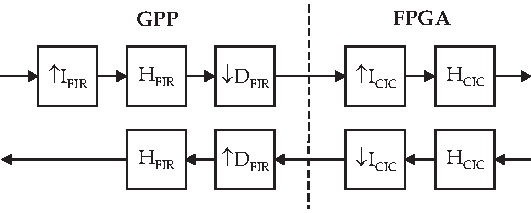
\includegraphics{../kapitel04/figures/tetra_rx_sampling_USRP.pdf}
%	\caption{Overview of the resampling on the USRP}
%	\label{fig:tetra_rx_sampling_USRP}
%\end{figure}
%
%
%\subsection{Resampling}
%\index{Resampling}
%The resampling on the transmit side is done in two stages, one interpolation on the FPGA and one resampling on the GPP. The following objectives have to be achieved:
%
%\begin{itemize}
%	\item The sampling rate must be converted from $f_\text{sym}$ to $f_s$.
%	\item The pulse shaping of the transmitter must be equal to the frequency response of a root raised cosine filter.
%	\item The conditions for the TETRA spectrum mask must be maintained.
%\end{itemize}
%
%As indicated in the previous section, the interpolation filter on the FPGA can be realized as a \ac{CIC} filter\index{CIC filter} with a frequency response as follows:
%
%\begin{equation}
%	G_\text{CIC}(f) = \left[\frac{\sin\left(\pi f T_{\text{sym}} \frac{D_\text{FIR}}{I_\text{CIC}}\right)}{\sin\left(\pi f T_{\text{sym}} \frac{D_\text{FIR}}{I_\text{FIR}\cdot I_\text{CIC}}\right)}\right]^{N_{\text{CIC}}}
%	\label{eq:g_cic_f}
%\end{equation}
%The parameters for the resampling are already given, therefore the number of stages $N_\text{CIC}$ remains as the only parameter to configure this filter. To ensure that the overall frequency response of the system is equal to a root raised cosine, a \ac{CIC} compensation filter has to be implemented on the GPP. The frequency response for this filter $G_{\text{FIR}}$ on the GPP can be calculated by
%
%\begin{equation}
%	G_{\text{FIR}}(f) = \frac{G_{\text{RRC}}(f)}{G_{\text{CIC}}(f)}\;,
%\end{equation}
%
%where $G_{\text{RRC}}(f)$ is the frequency response of an RRC filter as described in (\ref{eq:g_rrc_f}) and $G_{\text{CIC}}(f)$ is the frequency responses for the \ac{CIC} filter as described in (\ref{eq:g_cic_f}).
%
%A root raised cosine filter is also a low pass filter where the pass band depends on the roll-off factor\index{Roll-off factor} $\alpha$. Therefore, the relation between interpolation and decimation on the FIR filters should fulfill the following condition: 
%
%\begin{equation}
%\frac{I_{FIR}}{D_{FIR}} \geq 1 + \alpha
%\label{eq:crit}
%\end{equation}
%
%The filters are realized digitally on reconfigurable logic or processors. From the discrete time impulse response, the frequency response can be calculated for the CIC filter as follows:
%
%\begin{equation}
%	H_\text{CIC}(f) = \sum_{n=-\infty}^{\infty} G_\text{RRC} \left(f-n \frac{I_\text{FIR}\cdot I_\text{CIC}} {D_\text{FIR}\cdot T_\text{sym}}  \right)
%\end{equation}
%
%The frequency response of the discrete time filter $H_\text{FIR}(f)$ is given by
%
%\begin{equation}
%H_\text{FIR}(f) = \sum_{n=-\infty}^{\infty}G_\text{FIR}{\left(f-n \frac{I_\text{FIR}}{D_\text{FIR}}T_\text{sym} \right)} \text{si} \left( \pi f (2N_\text{FIR}+1) T_\text{sym} \right)\;.
%\end{equation}
%
%The decimation after filtering is included in the frequency response $H_\text{FIR}(f)$. The factor $N_\text{FIR}$  defines the length of the FIR filter, i.e. the number of filter taps. When combining these filters, the TETRA spectrum mask has to be considered in a way that the tolerance schemes, as given in table \ref{tab:TETRASpectrumMask} showing the maximum noise levels, are fulfilled .
%
%\begin{table}[htb]
%	\centering
%		\begin{tabular}{c|c}
%		\toprule
%		Frequency Offset & Maximum Noise Level \\
%		\midrule
%		\SI{25}{kHz} - \SI{50}{kHz}  & \SI{-55}{dBc} \\
%		\SI{50}{kHz} - \SI{100}{kHz}  & \SI{-70}{dBc} \\
%		\SI{100}{kHz} - \SI{250}{kHz}  & \SI{-75}{dBc} \\
%		\SI{250}{kHz} - \SI{5}{MHz}  & \SI{-80}{dBc} \\
%		$> \SI{5}{MHz}$  & \SI{-100}{dBc} \\
%		\bottomrule
%		\end{tabular}
%	\caption{TETRA spectrum mask\index{Spectrum mask} with the maximum noise levels in dependence of the frequency offset}
%	\label{tab:TETRASpectrumMask}
%\end{table}
%
%There are several ways of choosing the filter parameters to fulfill the above mentioned objectives. However, due to the fact that the CIC filters are the only signal processing elements on the FPGA, the interpolation factor of the CIC was chosen as high as possible to lower the interpolation factor on the GPP. The decimation factor $D_\text{FIR}$ was already defined in equation (\ref{eq:res_usrp}) to $D_\text{FIR}=9$. As follows, the smallest integer value of $I_\text{FIR}$ that holds the criteria (\ref{eq:crit}) is $I_\text{FIR}=16$. This determines the interpolation factor on the FPGA to $I_\text{CIC}=1000$. A CIC filter with $N_\text{CIC}=10$ stages suppresses the aliases of the RRC spectrum to be compliant with the tolerance scheme of the spectrum mask. With higher values of the filter length $N_\text{FIR}$, the spectrum gets closer to the RRC spectrum. According to section \ref{sec:PIM_TETRA}, the filter length was chosen as $N_\text{FIR}=6$. These parameters are summarized in table \ref{tab:usrp_res_par}. 
%
%
%\begin{table}[htb]
%	\centering
%		\begin{tabular}{c|c}
%		\toprule
%		Parameter & Value \\
%		\midrule
%		$N_\text{CIC}$  & 10 \\
%		$I_\text{CIC}$  & 1000 \\
%		$M_\text{CIC}$  & 1 \\
%		$I_\text{FIR}$  & 16 \\
%		$D_\text{FIR}$  & 9 \\
%		$N_\text{FIR}$  & 6 \\
%		\bottomrule
%		\end{tabular}
%	\caption{Parameters for the Resampling on the USRP}
%	\label{tab:usrp_res_par}
%\end{table}
%
%The frequency response of this system with RRC, CIC compensation and CIC filters is shown in figure \ref{fig:tetra_usrp_resampling} with reference to the TETRA spectrum mask and an optimum RRC filter.
%
%\begin{figure}[htb]
%	\centering
%		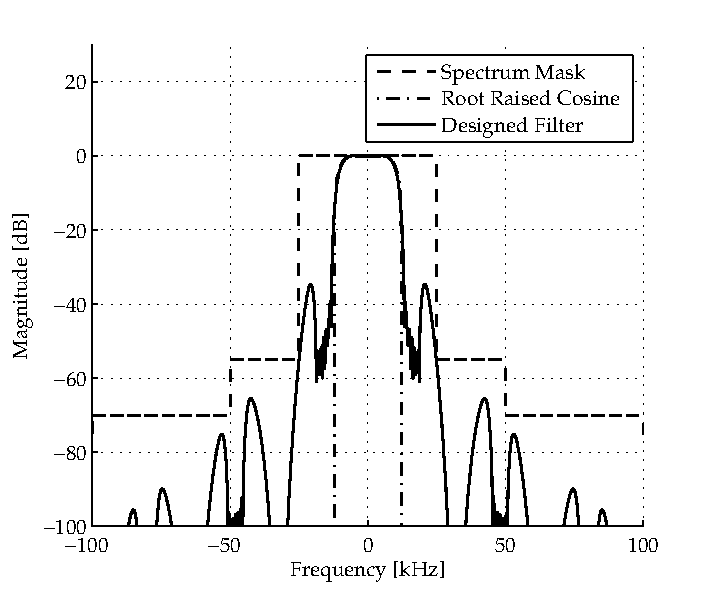
\includegraphics[width=1.00\textwidth]{../kapitel04/figures/tetra_usrp_resampling.pdf}
%	\caption{Designed filter, which fulfills the tolerance scheme of the TETRA spectrum mask}
%	\label{fig:tetra_usrp_resampling}
%\end{figure}
%
%
%It has to be mentioned that the impulse response of the filters for the receive path and the transmit path are identical. While the filter on the transmit path is the pulse shaping filter, the filter on the receive path is the matched filter. The values for the interpolation of the transmit side are now the values for the decimation on the receive side and vice versa, except for the decimation in the CIC filter which is double the interpolation factor on the transmit side. This is due to the different ADC and DAC rates. Another difference is that the filters on the receive side do not apply a decimation. The decimation in the last cascade is shifted to the timing synchronization, which is described in the following section.
%
%Table \ref{tab:usrp_fpga} shows the usage of \acp{LE} on the USRP's FPGA. It can be seen that \SI{92}{\%} of the provided space is used. Due to the fact that the decimation rate on the CIC receive filter twice the factor of the CIC transmit side, the usage for the receive side is higher. The usage of the overhead for buffers, \acl{DDC} or interfaces is given in table \ref{tab:MinimumAmountOfLogicElementsUsedInTheFPGA}. 
%
%\begin{table}
%	\centering
%		\begin{tabular}{c|c|c}
%		\toprule
%		\multirow{2}{*} {Cyclone} & \multicolumn{2} {c}{Logic Elements}\\
%				&	12060 &	100 \% \\
%		\midrule
%		Overhead			&	3895	&	32 \%	\\
%		CIC Rx				&	5374	&	45 \% \\		
%		CIC Tx				&	1871	& 16 \% \\
%		Sum						& 11140 & 93 \% \\
%		\bottomrule
%		\end{tabular}
%	\caption{Number of Logic Elements used in the FPGA}
%	\label{tab:usrp_fpga}
%\end{table}
%
%\subsection{Timing Synchronization}
%\index{Time synchronization}
%
%The timing synchronization is described in section \ref{sec:PIM_TETRA} but two parameters have still to be defined according to the underlying platform. These are the oversampling factor $I$ and the number of symbols that have a constant time offset $L$. The oversampling factor is given by the resampling filter design, which leads to
%\begin{equation*}
%I = I_\text{FIR} = 16\;.
%\end{equation*}
%
%The factor $L$ can be approximated by the timing error, caused by the oscillator on the USRP. According to section \ref{sec:USRP}, the frequency tolerance\index{Frequency tolerance} of the local oscillator is \SI{\pm 20}{ppm}. This leads to a maximum time shift of approximately one symbol interval in a three second period. Working with a frame length of $L =255$ symbols, as done in the \ac{PIM}, leads to a time shift of \SI{0.5}{\%} of the symbol time period after any frame. Therefore, no adaptation of the \ac{PIM} has to be taken into account and the timing error can be approximated as constant over one burst. Figure \ref{fig:usrp_time_offset} shows the normalized time offset for the USRP. The dashed lines are the maximum and minimum theoretical time offsets from the oscilator's instability while the solid line shows measured values on the USRP over one second. 
%
%\begin{figure}[htb]
%	\centering
%		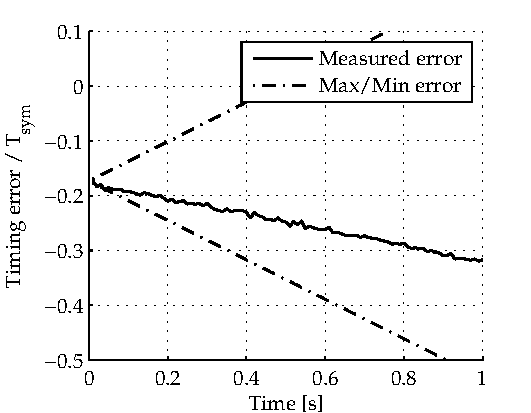
\includegraphics{../kapitel04/figures/usrp_time_offset.pdf}
%	\caption{Measured time offset with maximum and minimum conditions for the timing error}
%	\label{fig:usrp_time_offset}
%\end{figure}
%
%\subsection{Frequency Synchronization}
%\index{Frequency synchronization}
%The frequency offset is detected with the \textsc{Frequency Correction Field}\index{Frequency Correction Field} in the \textsc{Synchronization Downlink Burst} as described in section \ref{sec:PIM_TETRA}. However, due to the \SI{20}{ppm} inaccuracy of the oscillator the resulting frequency offset from the Flex400 daughter board can vary from \SI{\pm 8}{kHz} to \SI{\pm 10}{kHz}, depending on the carrier frequency. This value exceeds the maximum detectable frequency of the tracking which is \SI{9}{kHz}. Therefore, prior to tracking, a carrier acquisition\index{Carrier acquisition} scheme has to be applied on the \ac{USRP}. This scheme is according to the dual filter detector\index{Dual filter detector} as proposed in \cite{alberty}. The structure of this acquisition method is shown in figure \ref{fig:frequ_acq}. The band pass filters are placed symmetrically around the carrier frequency. If the energy of the signal filtered with the upper band pass is equal to the energy of the signal with the lower band pass, no frequency offset occurred. The two band pass filters and the spectrum of the TETRA signal are depicted in figure \ref{fig:freq_acq_design}. The magnitude square of the filter output can be seen as the energy of the filtered signal, whereas the error signal $e$ can be obtained by the subtraction of these two energies. 
%
%\begin{figure}[htb]
%	\centering
%		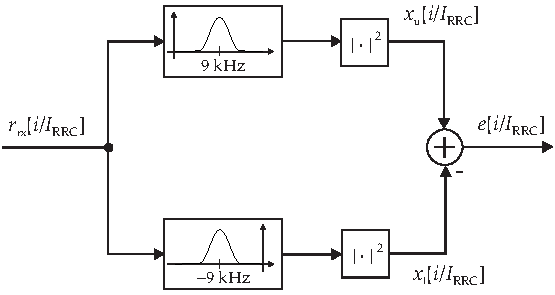
\includegraphics{../kapitel04/figures/frequ_acq.pdf}
%	\caption{Block diagram of the frequency acquisition}
%	\label{fig:frequ_acq}
%\end{figure}
%
%
%\begin{figure}[!htb]
%	\centering
%		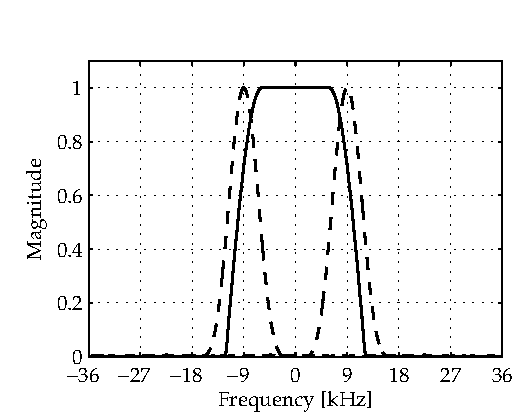
\includegraphics{../kapitel04/figures/freq_acq_design.pdf}
%	\caption{Illustration of the band pass filters and the raised cosine spectrum for the frequency acquisition}
%	\label{fig:freq_acq_design}
%\end{figure}
%
%\begin{figure}[!htb]
%	\centering
%		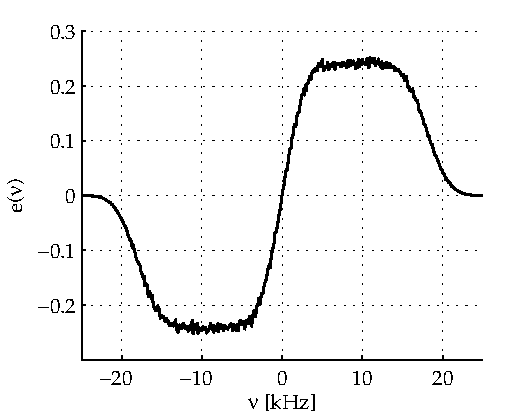
\includegraphics{../kapitel04/figures/freq_acq_error.pdf}
%	\caption{Error signal $e(\nu)$ of the dual filter detector in dependence on the frequency offset $\nu$}
%	\label{fig:freq_acq_error}
%\end{figure}
%
%The filters are designed as low pass filters and then transformed to band pass filters. For the low pass filters the window design was chosen in combination with a Hamming window. To ensure that the error signal has its highest values between \SI{8}{kHz} (frequency offsets lower than this value can be synchronized by the tracking) and \SI{10}{kHz} (this should be the highest frequency offset due to the oscillator inaccuracy), the center frequency was chosen to be \SI{9}{kHz}. Combined with the sampling rate of \SI{288}{kHz} at the input of the GPP, this leads to a tap length of multiples of 16. Figure \ref{fig:freq_acq_design} shows the frequency response of the band pass filters with the frequency response of the root raised cosine pulse shaping filter designed above. Figure \ref{fig:freq_acq_error} shows the error signal $e(\nu)$ in relation to the frequency offset $\nu$. 
%
%
%Large frequency offsets like \SI{\pm 10}{kHz} must only be synchronized at the start of the transmission. Therefore, the acquisition is only applied in the initialization phase of the receiver. The frequency synchronization as described in the \ac{PIM} controls that the frequency offset does not exceed the maximum value. The measurement of the current offset is performed for each received \textsc{Synchronization Downlink Burst} and the approximated frequency offset is saved until the next \textsc{Synchronization Downlink Burst} is detected. The following demodulation can be implemented as a subtraction of the previous phase value and the phase offset, which was evaluated by the frequency synchronization, from the current phase value.
%
%\subsection{MAC receiver}
%The whole frame synchronization as well as the receiver for the traffic channel and the \ac{AACH} are taken from the \ac{PIM} without any adaptations due to the signal processing. Changes that are made for measuring the processing time (varying of the data types, hand written versus generated code) are described in section \ref{sec:bench_gpp}.
%
%\section{Benchmarks for the waveform on the GPP}
%\label{sec:bench_gpp}
%
%The \ac{PSM} for the \ac{USRP} that was described in section \ref{sec:PSM_USRP} is transformed into C++ code and the execution time on a \ac{GPP} was measured. The processor is an Intel Core 2 Duo CPU (P8400) with a clock frequency of \SI{2.28}{GHz}. It was introduced in section \ref{sec:overhead} for the evaluation of the code generation overhead. The C++ code is compiled with \ac{VS} and executed on a Windows 7 operating system. All measurement results apply to one \textsc{Normal Downlink Burst}, which comprises 255 symbol periods.
%
%\begin{figure}[htb]
%	\centering
%		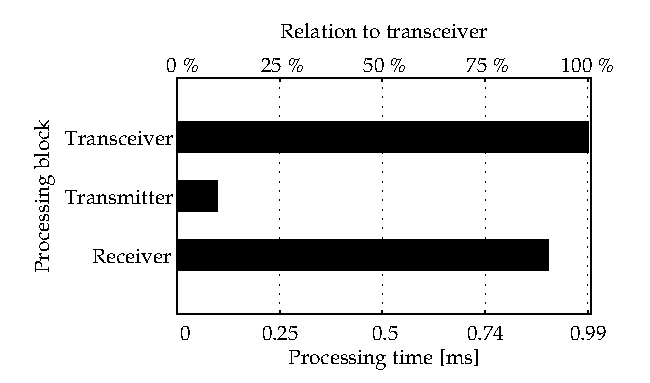
\includegraphics{../kapitel05/figures/bench_gpp_trx.pdf}
%	\caption{Comparison of the processing time for the transceiver, transmitter and receiver}
%	\label{fig:bench_gpp_trx}
%\end{figure}
%
%Figure \ref{fig:bench_gpp_trx} shows the processing time for the complete transceiver, which is \SI{0.99}{ms}. With the timing constraint of \SI{14.17}{ms} for one burst, only \SI{7}{\%} of the processor capacity is used. In this case the code was not optimized for the platform, except for the compiler flags. Figure \ref{fig:bench_gpp_trx} shows the processing time for one burst on the lower x-axis. To highlight the influence of the measured code segment on the whole system, the x-axis on the top is the relation of the processing time to the transceiver time. This form of representation is maintained for the following figures. In the transceiver measurements, the relation for the processing time from transmitter to receiver can be seen. Due to the increasing complexity for synchronization and decoding, the receiver consumes approximately ten times more processing time than the transmitter.
%
%
%In figure \ref{fig:bench_gpp_tx} the processing times of the different blocks in the transmitter are shown. They are separated in the \ac{MAC} blocks of the traffic channel (MAC TCH) and the broadcast channel (MAC AACH), the physical layer (PHY) and finally the sample rate conversion (SRC). The fact that the broadcast channel consumes only \SI{15.5}{\micro s} while the traffic channel consumes \SI{33}{\micro s} can be explained by the different frame lengths of both channels.
%
%The processing times of the functions inside the traffic channel are shown in figure \ref{fig:bench_gpp_tx}. 
%
%The broadcast channel MAC AACH consists of the following processing blocks: encoding and scrambling. The encoder is a Reed Muller encoder\index{Reed Muller code} as described in section \ref{sec:PIM_TETRA} with a processing time of \SI{15}{\micro s}. This is due to the slow realization of the matrix multiplication for binary values. However, this comprises only \SI{1.5}{\%} of the processing time for the transceiver, therefore no optimized version of the Reed Muller encoder was realized. The encoded data are scrambled with the same scrambling sequence used in the MAC TCH. This operation takes less than \SI{1}{\micro s}.
%
%
%\begin{figure}[htb]
%	\centering
%		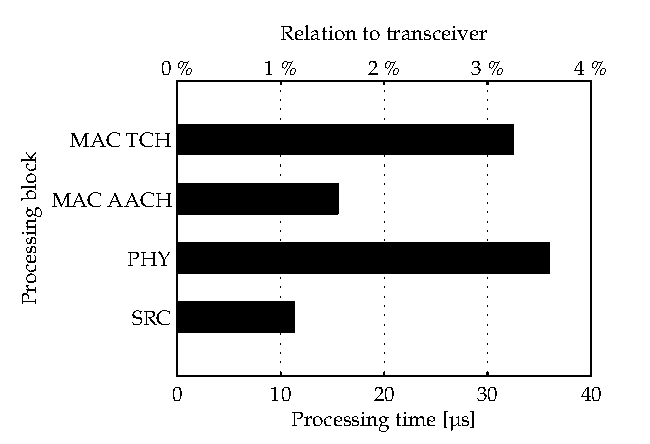
\includegraphics{../kapitel05/figures/bench_gpp_tx.pdf}
%	\caption{Comparison of the processing times in the transmitter}
%	\label{fig:bench_gpp_tx}
%\end{figure}
%
%
%The \ac{PHY} consists of the burst builder, which inserts training sequences and synchronization bursts in the data stream. It furthermore comprises the modulator for mapping the bits from the two logical channels (AACH and TCH) to symbols in the complex plane. With a processing time of \SI{36}{\micro s} this is the block with the highest time consumption in the transmitter. It can also be seen that the sample rate conversion can be applied very efficiently with the polyphase structure of the multirate filter. With the processor's clock frequency of \SI{2.28}{GHz} and the processing time for the \ac{SRC}\index{Sample rate conversion} of \SI{11.3}{\micro s}, approximately hundred clock cycles are used for the filtering and resampling of one complex symbol. This is a good value for a processor that is not optimized for digital signal processing. 
%
%Figure \ref{fig:bench_gpp_tx_tch} provides more details about the processing times of the signal processing blocks in the MAC TCH. The used traffic channel was the TCH/4.8 with an encoding rate $r = 292/432$. The \ac{RCPC}\index{Rate-Compatible punctured convolutional code} code needs \SI{20}{\micro s} and is the block with the highest time consumption. However, even if this block comprises puncturing and encoding, it uses only \SI{2}{\%} of the whole transceiver. The interleaving and the scrambling need \SI{5}{\micro s} and \SI{7}{\micro s}. This is due to the fact that both blocks are implemented regarding time and not memory. For the interleaving, an array is saved that provides mapping from the incoming data to the interleaved data. This vector is calculated at the initialization phase and has to be provided at run time. The implementation of the scrambling is similar. The scrambling sequence is calculated in the initialization phase and saved as a constant array during run time i.e. it is merely an exclusive disjunction of the incoming data with a constant array.
%
%\begin{figure}[htb]
%	\centering
%		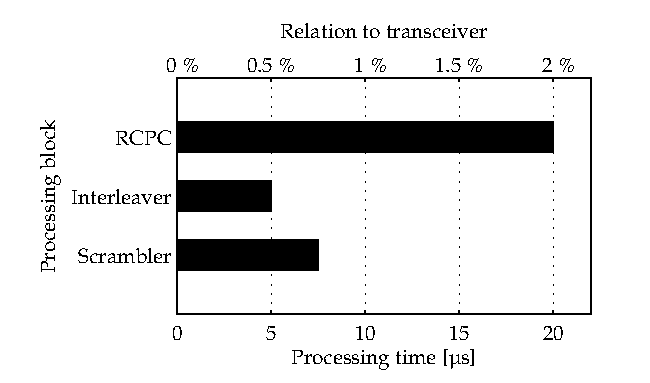
\includegraphics{../kapitel05/figures/bench_gpp_tx_tch.pdf}
%	\caption{Comparison of the processing times within the MAC TCH in the transmitter}
%	\label{fig:bench_gpp_tx_tch}
%\end{figure}
%
%Figure \ref{fig:bench_gpp_rx} shows the processing times of the various blocks in the receiver. It can be seen that the processing times are larger than the results for the transmitter in figure \ref{fig:bench_gpp_tx}. The receive side of the AACH receiver consists of a syndrome decoder and descrambling. The relatively short time for this processing block is due to the relaxed non-optimal implementation that corrects only one error and the short frame length. The \ac{SRC} takes, with \SI{110}{\micro s}, about eight times more than the \ac{SRC} in the transmitter. This is due to the fact that no decimation is applied after filtering. The interpolated values are sent to the timing error detector, which triggers the downsampling. Similar to the \ac{SRC}\index{Sample rate conversion}, the \ac{PHY} on the receive side consumes with \SI{368}{\micro s} about ten times more than the physical layer in the transmitter. In this case, this is due to the various synchronization schemes that must be applied.
%
%\begin{figure}[h!!]
%	\centering
%		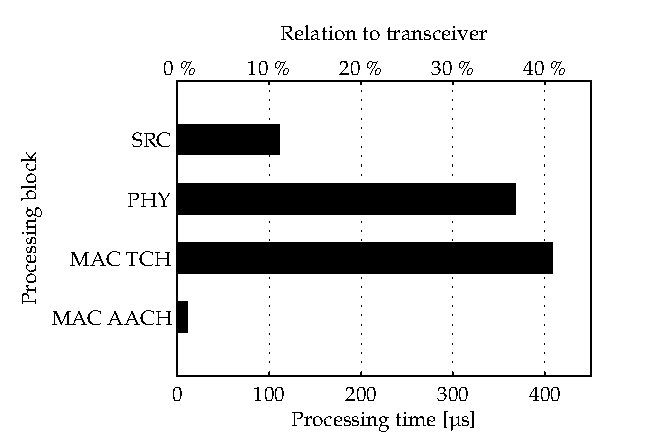
\includegraphics{../kapitel05/figures/bench_gpp_rx.pdf}
%	\caption{Comparison of the processing times in the receiver}
%	\label{fig:bench_gpp_rx}
%\end{figure}
%
%In figure \ref{fig:bench_gpp_rx_phy}, the processing times of the blocks in the PHY are shown. While the transmitting part of the PHY consists only of a burst builder and a modulator, the receiving part of the PHY must correct time, frequency and symbol offsets. In these synchronization schemes, the timing error correction is the most simple regarding the processing time of \SI{50}{\micro s}. The frequency error correction applies two correlations to find the synchronization burst and is therefore more complex with \SI{146}{\micro s}. The frame synchronization realizes two buffers that are filled when training sequences are found inside a vector. These buffers are transmitted to the TCH and AACH receiver.
% 
%\begin{figure}[htb]
%	\centering
%		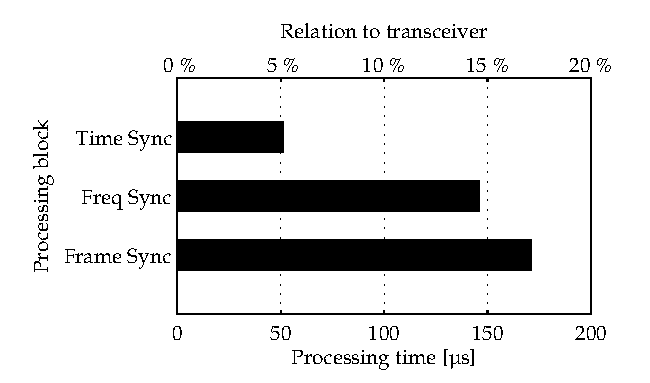
\includegraphics{../kapitel05/figures/bench_gpp_rx_phy.pdf}
%	\caption{Comparison of the processing times within the PHY in the receiver}
%	\label{fig:bench_gpp_rx_phy}
%\end{figure}
%
%
%The measurements of the processing time for the MAC TCH receiver are presented in figure \ref{fig:bench_gpp_rx_tch}. It is obvious that the Viterbi decoding\index{Viterbi decoding} is the bottleneck for the transceiver with \SI{388}{\micro s}, which makes about \SI{40}{\%} of the processing time for the complete system. In relation to that, the descrambling and the de-interleaving can be almost ignored. The same block is used for descrambling as for scrambling, therefore the times are equal. The same is true for the de-interleaver, except for the different entries in the mapping vector.
%
%\begin{figure}[!!h]
%	\centering
%		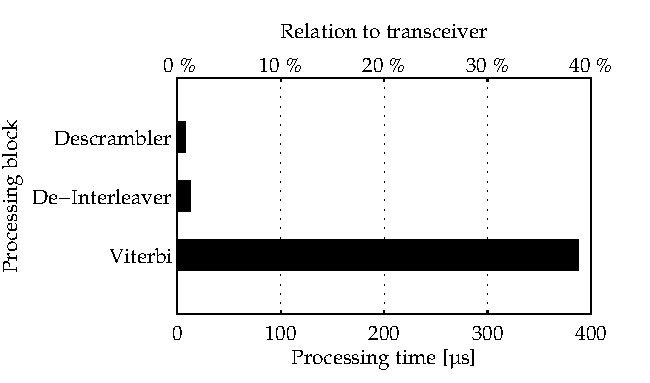
\includegraphics{../kapitel05/figures/bench_gpp_rx_tch.pdf}
%	\caption{Comparison of the processing times within the MAC TCH in the receiver}
%	\label{fig:bench_gpp_rx_tch}
%\end{figure}
%
%
%\section{Platform Specific Model for the SFF SDR}
%
%\subsection{Separation on different Processing Units}
%The processing performance of the SFF differs from the USRP in so far as the FPGA on the SFF provides more logical resources and additional hardware multipliers\index{Hardware multiplier}. This leads to the possibility to shift more signal processing to the FPGA, as done in the \ac{PSM} for the USRP. Another difference of this platform to the USRP is the DSP. Even if it provides an optimized hardware architecture for digital signal processing, its clock frequency of \SI{594}{MHz} is approximately four times lower than the \ac{GPP} used in combination with the \ac{USRP}. Further, the cache size makes with \SI{172}{kB} only \SI{2}{\%} of the cache size on the GPP. The third major difference is the possibility of the clock distribution on the \ac{DCM}. This means that the sampling rate of the data converters can be configured in a range between \SI{25}{MHz} and \SI{125}{MHz} as described in section \ref{sec:SFF}.
%
%The choice of the sampling rate depends on two parameters: the symbol rate $f_\text{sym}$ that should be achieved and the \ac{IF} $f_\text{IF}$ that is needed for downconversion. The sampling rate can be calculated as follows:
%
%\begin{equation}
%f_\text{DAC} = k f_\text{IF} = I_\text{FIR} I_\text{CIC} f_\text{sym}\;,
%\end{equation}
%
%where $k$ is an integer not smaller than two, and $I_\text{FIR}$ and $I_\text{CIC}$ are the upsampling factors of two cascaded filters, similar to the resampling filters designed in the \ac{PSM} for the \ac{USRP}. The \ac{CIC} filter\index{CIC filter} is  processing the high upsampling rates while the \ac{FIR} filter compensates the non exact flat pass band in combination with the \ac{RRC} pulse shaping. Due to the fact that the clock can be adjusted to a multiple of the symbol rate no more decimation is needed.
%
%An ideal relation between \ac{IF}\index{Intermediate frequency} and clock rate would be a factor of four, where the \ac{IF} would then only consist of additions and subtractions. With this configuration the \ac{IF} of \SI{30}{MHz} on the SFF would lead to a clock rate of \SI{120}{MHz}. Even if the clock distribution circuit is able to handle this frequency, it is not a multiple of the symbol rate of \SI{18}{kHz}. This would demand a resampling filter as designed in the \ac{PSM} for the \ac{USRP}. The advantage of the relaxed implementation of the down-conversion would be on the cost of an additional filter for the resampling in the DSP.
%
%A good compromise would be a sampling rate of \SI{90}{MHz}. With this clock frequency the down-conversion can be implemented by the multiplication of the signal with three constants for the in-phase component and another three constants for the quadrature component which can be saved easily in a \ac{LUT}\index{Lookup table}. This sampling rate would also define the upsampling factor of the system as follows:
%\begin{equation}
%I_\text{CIC} \cdot I_\text{FIR} = \frac{f_\text{ADC}}{f_\text{sym}} =  \frac{\SI{90}{MHz}}{\SI{18}{kHz}} = 5000
%\end{equation}
%The sample rate conversion and pulse shaping on the FPGA does not only reduce the load of the \ac{DSP} but also the load of the bus between DSP and FPGA. To ensure that the bus on the SFF runs at the same speed for transmit and receive path, the time synchronization has to be implemented in the FPGA. This leads to a separation as shown in figure \ref{fig:sep_sff}.
%
%
%\begin{figure}[htb]
%	\centering
%		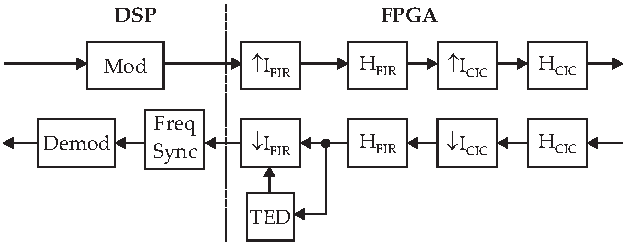
\includegraphics{../kapitel04/figures/sep_sff.pdf}
%	\caption{Separation of the processing function in the SFF between DSP and FPGA}
%	\label{fig:sep_sff}
%\end{figure}
%
%\subsection{Sample Rate Conversion}
%\index{Sample rate conversion}
%The conversion from symbol rate to sampling rate of the data converters consists only of interpolation filters, running on the FPGA. Similar to the USRP model, two interpolation filters should be designed that hold the conditions of the TETRA spectrum mask in a cascaded mode. In the receive path only one decimation filter shall be applied. After the adherent matched filter, the oversampled data are sent to the timing error detector, which implements the final decimation regarding the calculated timing error. Therefore, the filters are designed in a way that, in combination with the timing synchronization, the FPGA resources are used to the maximum.
%The filter parameters are listed in table \ref{tab:sff_res_par}. The frequency response of the interpolation filter is shown in figure \ref{fig:tetra_sff_resampling}. For a reference also the TETRA spectrum mask and an ideal root raised cosine transmit filter is represented.
%
%\begin{table}[htb]
%	\centering
%		\begin{tabular}{c|c}
%		\toprule
%		Parameter & Value \\
%		\midrule
%		$N_\text{CIC}$  & 6 \\
%		$I_\text{CIC}$  & 625 \\
%		$M_\text{CIC}$  & 6 \\
%		$I_\text{FIR}$  & 8 \\
%		$N_\text{FIR}$  & 4 \\
%		\bottomrule
%		\end{tabular}
%	\caption{Parameters for the interpolation on the SFF}
%	\label{tab:sff_res_par}
%\end{table}
%
%\begin{figure}[htb]
%	\centering
%		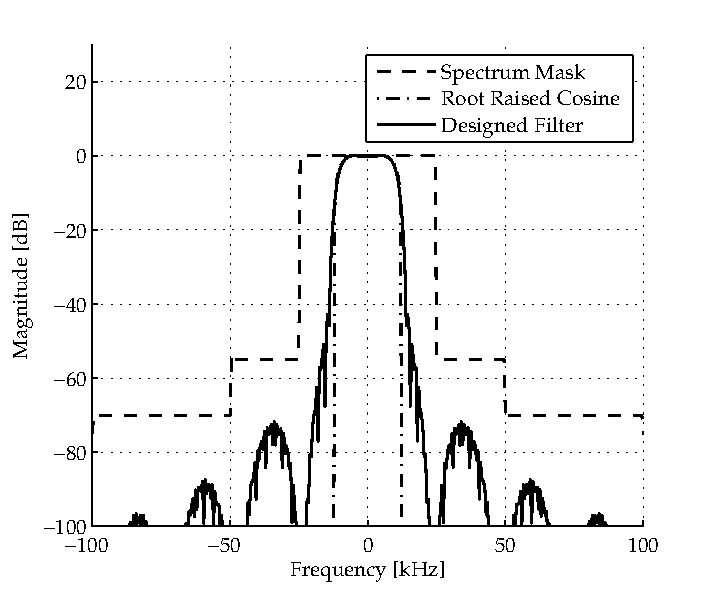
\includegraphics[width=1.00\textwidth]{../kapitel04/figures/tetra_sff_resampling.pdf}
%	\caption{Frequency response of the interpolation filter on the SFF with respect to the TETRA spectrum mask and an ideal RRC filter}
%	\label{fig:tetra_sff_resampling}
%\end{figure}
%
%
%\subsection{Timing error synchronization}
%Due to the shift of the timing error synchronization from the GPP to the FPGA, the design has to be adapted from a floating point, frame based implementation to a fixed point, sample based design. The sine and cosine functions, needed for the calculation of the Fourier coefficients, must be implemented with a lookup table. This table must only hold $I_\text{FIR}$ values. With the results from the previous section, this would mean eight values for the sine and another eight values for the cosine. This can be optimized with only one lookup table and shifted accesses for the sine and the cosine waves. The Fourier coefficients can be calculated by the multiplication of the squared magnitude with the sine waves. Figure \ref{fig:sff_ted} gives an overview of the timing error detector on the FPGA. 
%
%\begin{figure}[htb]
%	\centering
%		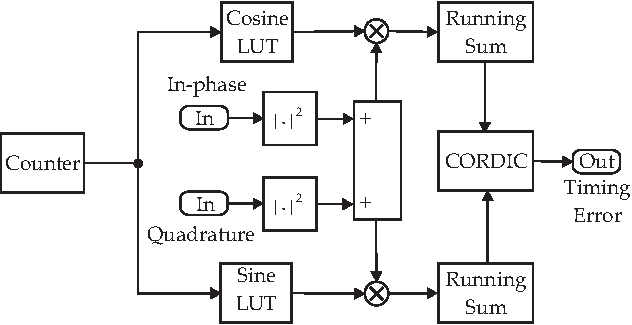
\includegraphics[]{../kapitel04/figures/sff_ted.pdf}
%	\caption{Overview of the fixed point realization of the timing error detector for the FPGA}
%	\label{fig:sff_ted}
%\end{figure}
%
%It is assumed that the timing error is constant over $L$ symbol intervals. To avoid random peaks in the timing error signal a moving average filter with length $L \cdot I_\text{RRC}$ is implemented. By realization of the filter in an FIR form, the number of taps grows with the length of $L\cdot I_\text{RRC}$. To circumvent this, the FIR filter can be transformed to an IIR filter with the use of the geometric series. The z-transformation of a moving average filter can simply be described as follows:
%\begin{eqnarray}
%H(z) 	&=& \sum_{i=0}^{L\cdot I_\text{RRC}-1}{z^{-i}} \\
%			&=& \frac{1-z^{-L\cdot I_\text{RRC}}}{1-z^{-1}}
%\end{eqnarray}
%
%The increasing number of taps for the FIR filter is now transformed in a delay component. The resulting filter can be designed efficiently in hardware with only two adders and two delay lines. The block diagram of the efficient calculation is shown in figure \ref{fig:sff_rs}.
%
%\begin{figure}[htb]
%	\centering
%		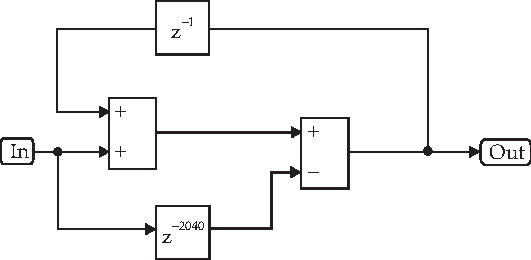
\includegraphics[]{../kapitel04/figures/sff_running_sum.pdf}
%	\caption{Hardware efficient implementation of a running sum}
%	\label{fig:sff_rs}
%\end{figure}
%
%The last block in the timing error detector is the transformation from real ($x$) and imaginary ($y$) parts of the symbol to its angle ($\varphi$). Therefore, an implementation of an inverse tangent function can be applied. This is done by a \ac{CORDIC}\index{CORDIC} algorithmic element as described in \cite{cordic}. Due to the fact that real and imaginary parts of the complex symbol are given, the vectoring computing mode is used. Therefore, a vector of $N_{\varphi}$ angle values $\theta[i]$ is saved in the initialization phase to rotate the phase:
%
%\begin{equation}
%\theta[i] = \text{atan} \left(2^{-i}\right) \quad \text{for} \quad 1 \leq i \leq N_{\varphi}
%\end{equation}
%
%As follows, the iterative process to calculate the phase $\varphi$ can be described by
%\begin{eqnarray}
%\varphi[i+1]	&=& \varphi[i] + \text{sgn} \left(y[i] \right) \cdot \theta[i]\;, \\ 
%x[i+1]				&=& x[i] + \text{sgn} \left(y[i] \right) \cdot 2^{-i}y[i]\;, \\ 
%y[i+1]				&=& y[i] - \text{sgn} \left(y[i] \right) \cdot 2^{-i}x[i]\;.
%\end{eqnarray}
%
%This process assumes a complex value in the first quadrant of the complex plane. If this is not the case, the quadrant can be defined by the sign bits of the real and imaginary part and a phase offset can be added. Another difference to an original CORDIC algorithm is the missing scaling factor but this is no problem since only the resulting angle is of interest. The implementation of the sign function consist of an extraction of the sign bit of the imaginary part which triggers an adder. Furthermore, the multiplication by the factors of $2^{-i}$ are only bit shifts of $i$. The upper bound of $N_{\varphi}$ is given by the used word length of 16.
%
%The timing offset $\epsilon$ can be calculated with the evaluated phase through scaling and rounding to the nearest integer:
%\begin{equation}
%\epsilon[k] =\left\lfloor  \frac{\varphi[k]}{2\pi} \cdot I_\text{FIR} + 0.5 \right\rfloor
%\end{equation}
%
%The maximum error of the CORDIC algorithm occurs if the correct phase is found at the step $i=N_{\varphi}-1$. Then, the phase rotates with the maximum angle, which can be described by
%\begin{equation}
%\theta[N_\varphi-1] = \text{atan}\left(2^{-\left(N_\varphi-1\right)} \right)\;.
%\end{equation}
%
%Due to rounding, the accuracy of the phase with the CORDIC algorithm should be small against the following decimation, which can be described by the following condition:
%\begin{equation}
%\frac{\theta[N_\varphi-1]}{2\pi} \cdot I_\text{FIR}  \ll 1
%\label{eq:cordic_acc}
%\end{equation}
%
%Figure \ref{fig:cordic_error} shows the error value from the left hand side of inequality (\ref{eq:cordic_acc}) in dependence to the number of steps in the CORDIC algorithm $N_\varphi$. It can be seen that seven iterations for the CORDIC algorithm already fulfills this condition.
%
%
%\begin{figure}[htb]
%	\centering
%		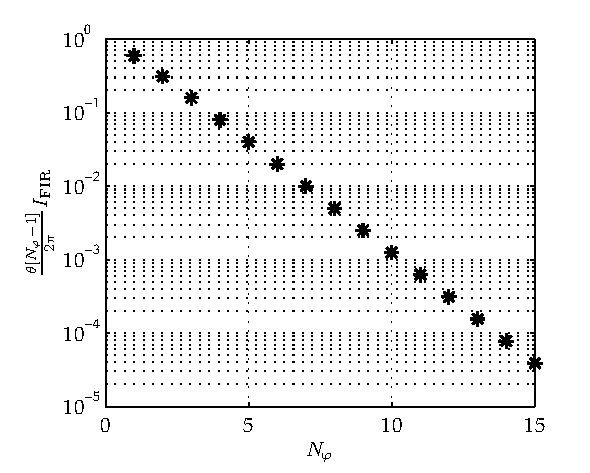
\includegraphics{../kapitel04/figures/cordic_error.pdf}
%	\caption{Error for the phase calculation in relation to the number of steps $N_\varphi$, assuming an interpolation factor of $I_\text{FIR}=8$}
%	\label{fig:cordic_error}
%\end{figure}
%
%The resulting phase triggers the downsampling. The symbols with the corrected timing offset are sent to the DSP at the TETRA symbol rate of \SI{18}{kHz}.
%
%
%\subsection{PSM on the DSP}
%The porting of the waveform from USRP to SFF should be done with a minimum effort of rewriting code, the majority of the \ac{PSM} for USRP's GPP shall be used at the DSP on the SFF. The differences are, as already mentioned in the previous sections, the sample rate conversion and the time synchronization, which was shifted to the FPGA. In chapter \ref{sec:bench_dsp} the operations are described that must be tuned in order to get an operating waveform. No frequency acquisition has to be applied due to the precise oscillator with an accuracy of \SI{1}{ppm}, which leads to a maximum frequency offset of \SI{\pm 500}{Hz}.
%
%
%\section{Benchmarks for the waveform on the DSP}
%\label{sec:bench_dsp}
%The \ac{PSM} for the USRP can be ported to the SFF by shifting the time synchronization and the pulse shaping to the FPGA. This means these blocks have to be deleted from the DSP side. By measuring the processing time of the waveform, one single burst is in the range of seconds. It could be shown that the processing time of the code causes less problems than the memory allocation. Every memory section of the code must be placed on the external SDRAM, when the \ac{PSM}, originally intended for a \ac{GPP} is inserted. This needs several read and write operations, for example: to load the section of the SDRAM into the internal cache, to process these data and to write it back to the external memory.
%
%
%\begin{table}[h]
%\centering
%\begin{tabular}{c|cc}
%\toprule
% 			& Generated & Hand-written \\
% \midrule
% Processing time			& \SI{120}{ms}	& \SI{248}{\micro s}	\\
% Level 1 memory 	& \SI{0}{kB}		& \SI{1.04}{kB} \\
% Level 2 memory 	& \SI{0}{kB}		& \SI{11.1}{kB} \\
% SDRAM						& \SI{54.8}{kB}	& \SI{0}{kB} \\
% \bottomrule			
%\end{tabular}
%\caption{Comparison of processing times and memory allocation for generated and hand-written part of the transmitter}
%\label{tab:mac_tch_bench}
%\end{table}
%
%
%The difference between processing on the SDRAM and processing on the L1 and L2 memory sections can be seen with the following example. The MAC section of the transmitter has been rewritten in C code and compared with generated code. While the generated code was executed on the external SDRAM, the hand written code was executed on the internal cache of the processor. The results are shown in table \ref{tab:mac_tch_bench}. It can be seen that the generated code needs approximately 500 times more processing time than the hand-written code. This is mainly caused by the slow read and write accesses of the external memory.
%
%\begin{figure}[htb]
%	\centering
%		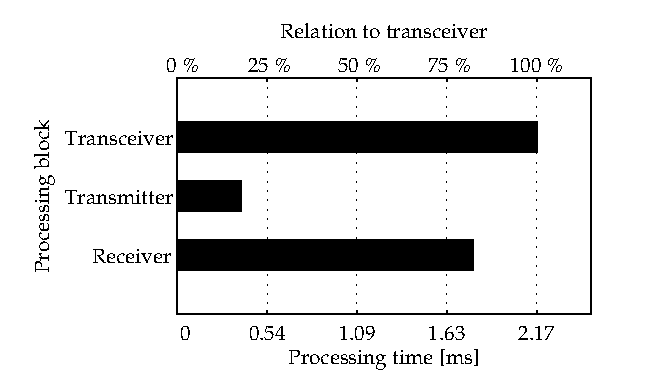
\includegraphics{../kapitel05/figures/bench_dsp_trx.pdf}
%	\caption{Comparison of the processing times of the transmitter, receiver and transceiver for the DSP}
%	\label{fig:bench_dsp_trx}
%\end{figure}
%
%The generated code creates a lot of arrays for the signal processing where especially for the puncturing an array with a length of 1168 is created. In this array for puncturing the positions of the coded bits that can be dropped are contained. This is the same for the interleaving, where an array is created with the position of the interleaved data. While these methods work really fast, they consume a lot of memory. For a GPP with an internal cache of \SI{8}{MB} this is not a problem. The DSP however, has to shift these sections to the external SDRAM, where it needs much more time. To compare the memory usage, the hand-written code was optimized for memory consumption but not for speed. This means the punctured channel encoder and the interleaver have been combined in one function. No bits are encoded that would be dropped due to the puncturing, and the encoded bits are immediately shifted to the right position as specified through the interleaving scheme. The code is shown in appendix \ref{sec:app_01}. This was also done for the scrambling of the data. The code for the optimized scrambling is shown in appendix \ref{sec:app_02}. Due to to the register length of 32, the whole register can be calculated with one single integer value that has a size of four bytes. The used memory of both functions is also shown in table \ref{tab:mac_tch_bench}. Compared to the memory usage of the generated code with \SI{54.8}{kB}, the optimized code consumes \SI{12.1}{kB}. The reason why the generated code was placed on the SDRAM is the better comparability to the whole transceiver. By generating the code for the transceiver, it has to be placed on the external memory. This is not the same for the hand written code. Due to the optimization options, it is possible to place the code for the complete transceiver on the internal cache.  
%
%Figure \ref{fig:bench_dsp_trx} shows the relation of the processing times between transmitter and receiver. The receiver consumes approximately \SI{80}{\%} of the processing time for the complete transceiver. This is similar to the results for the GPP from section \ref{sec:bench_gpp} although the time synchronization as well as the resampling was moved to the \ac{FPGA}. However, the processing time for the complete transceiver is with \SI{2.17}{ms} approximately twice the time of the code running on the \ac{GPP}.
%
%\begin{figure}[h]
%	\centering
%		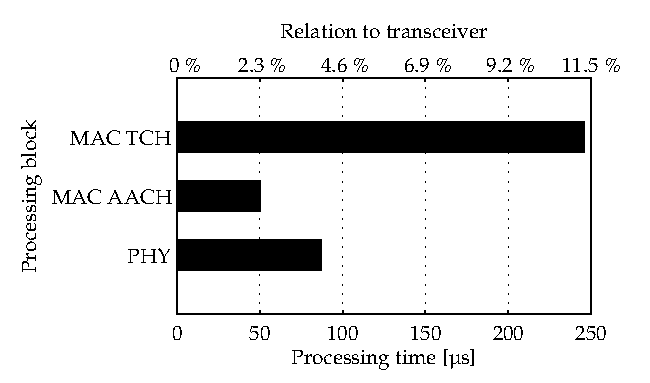
\includegraphics{../kapitel05/figures/bench_dsp_tx.pdf}
%	\caption{Comparison of the processing times within the transmitter on the DSP}
%	\label{fig:bench_dsp_tx}
%\end{figure}
%
%
%\begin{figure}[h]
%	\centering
%		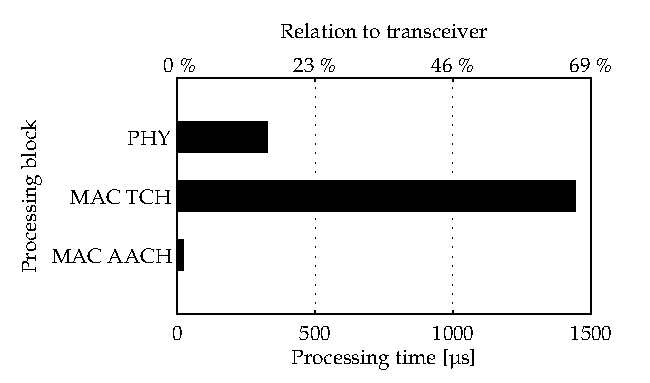
\includegraphics{../kapitel05/figures/bench_dsp_rx.pdf}
%	\caption{Comparison of the processing times within the receiver on the DSP}
%	\label{fig:bench_dsp_rx}
%\end{figure}
%
%
%The transmitter is split in three parts as shown in figure \ref{fig:bench_dsp_tx}: The PHY, the traffic channel MAC TCH and the broadcast channel MAC AACH. The processing time for the TCH is already known from table \ref{tab:mac_tch_bench}. Compared to the results from figure \ref{fig:bench_gpp_tx} the MAC TX block needs more time. This is due to the fact that the code is now optimized for memory and therefore slower than a code that is optimized for speed. The processing blocks PHY and MAC AACH were not changed.
%
%Figure \ref{fig:bench_dsp_rx} shows the processing times of the functions on the receive side. It can be seen that the traffic channel is the block that consumes the most processing time. The difference to the other blocks have been increased in comparison to figure \ref{fig:bench_gpp_rx}. This is due to the fact that the timing synchronization as well as the decimation at the receive side was realized on the FPGA. 
%
%The both remaining blocks on the physical layer need with \SI{191}{\micro s} for the frequency synchronization and \SI{135}{\micro s} for the frame synchronization approximately similar processing times as on the GPP. These processing times are shown in figure \ref{fig:bench_dsp_rx_phy}. 
%
%\begin{figure}[h!!]
%	\centering
%		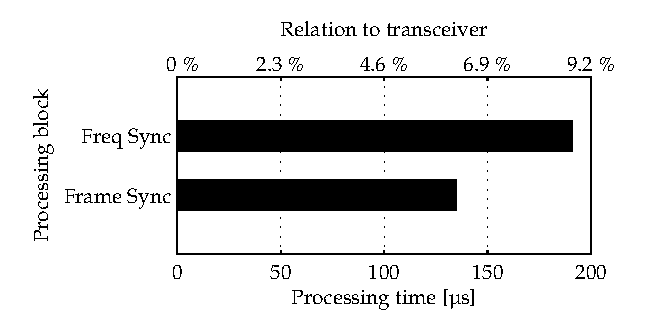
\includegraphics{../kapitel05/figures/bench_dsp_rx_phy.pdf}
%	\caption{Comparison of the processing times within the PHY in the receiver}
%	\label{fig:bench_dsp_rx_phy}
%\end{figure}
%
%Figure \ref{fig:bench_dsp_rx_tch} shows the reason for the large processing time of the MAC receiver. The Viterbi algorithm consumes approximately \SI{65}{\%} of the processing time of the whole transceiver. To circumvent this problem, modern DSPs provide hard wired Viterbi accelerators. Unfortunately the DM6446 does not provide those accelerators. Therefore, the decoder has to be implemented in software and remains the bottleneck of the complete system as already shown in the results for the GPP.  
%
%\begin{figure}[h!!]
%	\centering
%		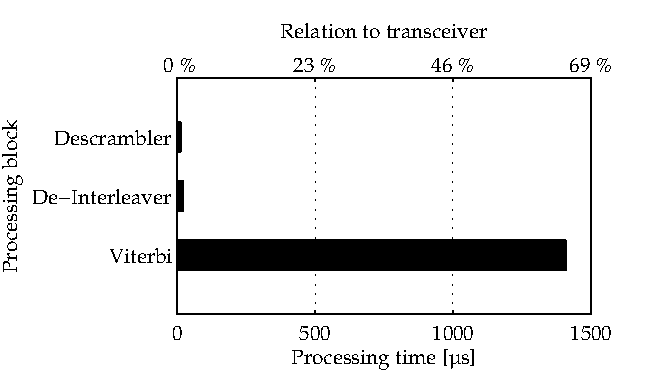
\includegraphics{../kapitel05/figures/bench_dsp_rx_tch.pdf}
%	\caption{Comparison of the processing times within the MAC TCH in the receiver}
%	\label{fig:bench_dsp_rx_tch}
%\end{figure}
%
%\section{Interoperability Tests}
%\index{Interoperability}
%
%A signal generator and a analyzer were used as a reference to prove that the transmitting and receiving behavior of the generated waveforms for USRP and SFF are like TETRA signals. To test the transmit function, the signals from USRP and SFF were evaluated with a Rohde \& Schwarz FSQ8 signal analyzer. As shown in figure \ref{fig:screenshot_tetra_01}, the signals are processed with a special software that shows the training sequence as well as the signal constellation and the modulation accuracy.
%
%\begin{figure}[htb]
%	\centering
%		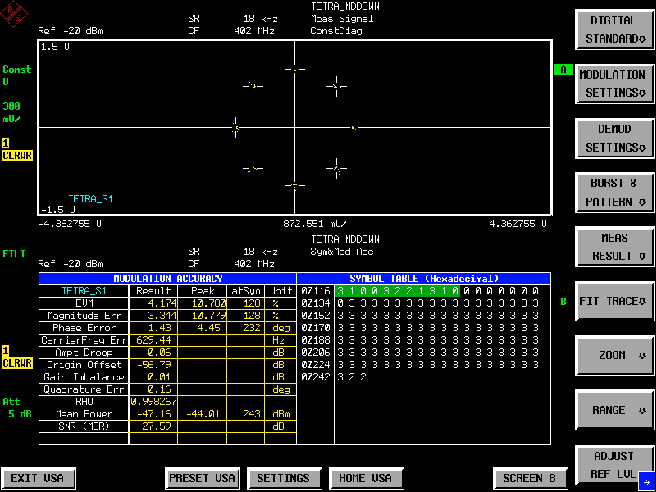
\includegraphics[width=1.00\textwidth]{../kapitel05/figures/screenshot_tetra_01.pdf}
%		\caption{Received TETRA signal from the SFF, evaluated with an FSQ8}
%	\label{fig:screenshot_tetra_01}
%\end{figure}
%
%To test the receive path on USRP and SFF SDR, TETRA signals were generated with a Rohde \& Schwarz SMU200 signal generator. USRP and SFF were tuned on a carrier frequency of \SI{402}{MHz} and decoded the \textsc{Normal Downlink Burst} correctly. To ensure that the transmissions from USRP to SFF and vice versa works correctly, the transmit and receive functions were tested in both directions and the decoded data were compared for errors. However, no errors occurred due to the close distance between transmitter and receiver. The setup for the demonstration of the waveform is shown in figure \ref{fig:Interoperability}. The USRP is on the left hand side with a laptop for the signal processing. The SFF is on the right hand side of the picture. The desktop is only used for configuration and does not process any radio signals. The measurement equipment is in the center of the picture. The lower device is the FSQ8 signal analyzer and the upper device is the SMU200A signal generator.
%
%\begin{figure}[htb]
%	\centering
%		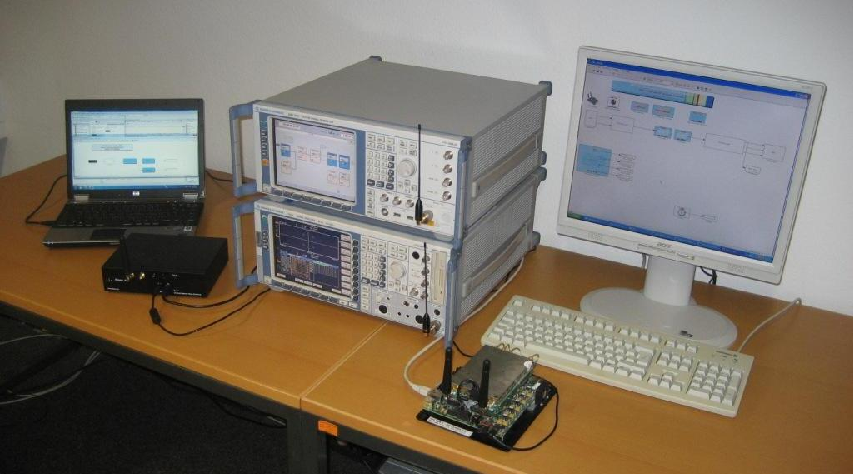
\includegraphics[width=1.00\textwidth]{../kapitel05/figures/Interoperability_demo_small.pdf}
%	\caption{Measurement setup for the TETRA waveform testing}
%	\label{fig:Interoperability}
%\end{figure}
%
%
%
%
%
%
